% (c) 2012 - 2014 Dimitrios Vrettos - d.vrettos@gmail.com
% (c) 2012 Silvia Cibola - silvia.cibola@gmail.com

\chapter{Polinomi}
\section{Definizioni fondamentali}

\begin{definizione}
Un \emph{polinomio} è un'espressione algebrica letterale che consiste in una somma algebrica di monomi.
\end{definizione}

\begin{exrig}
\begin{esempio}
Sono polinomi:~$6a+2b$, $\:5a^2b+3b^2$, $\:6x^2-5y^2x-1$, $\:7ab-2a^2b^3+4$.
\end{esempio}
\end{exrig}

Se tra i termini di un polinomio non sono presenti monomi simili, il polinomio si dice in \emph{forma normale} o
\emph{ridotto}; se al contrario si presentano dei termini simili, possiamo eseguire la riduzione del polinomio
sommando algebricamente i termini simili. Tutti i polinomi sono quindi riducibili in forma normale.

Un polinomio in forma normale può presentare, tra i suoi termini, un monomio di grado~0 che viene
comunemente chiamato \emph{termine noto}.

\begin{exrig}
\begin{esempio}
Il polinomio~$3ab+b^2−2ba+4−6ab^2+5b^2$ ridotto in forma normale diventa~$ab+6b^2−6ab^2+4$. Il termine noto è~$4$.
\end{esempio}
\end{exrig}

\ovalbox{\risolvi\ref{ese:11.1}}\vspazio

Un polinomio può anche essere costituito da un unico termine, pertanto un monomio è anche un polinomio.
Un polinomio che, ridotto in forma normale, è somma algebrica di due, tre, quattro monomi non nulli si dice
rispettivamente binomio, trinomio, quadrinomio.

\begin{exrig}
\begin{esempio}
Binomi, trinomi, quadrinomi.
\begin{enumeratea}
\item $xy−5x^3y^2$ è un binomio;
\item $3ab^2 +a−4a^3$ è un trinomio;
\item $a−6ab^2+3ab−5b$ è un quadrinomio.
\end{enumeratea}
\end{esempio}
\end{exrig}

\begin{definizione}
Due polinomi, ridotti in forma normale, formati da termini uguali si dicono \emph{uguali}, più precisamente vale il \emph{principio di identità dei polinomi}:
due polinomi~$p(x)$ e~$q(x)$ sono uguali se, e solo se, sono uguali
i coefficienti dei rispettivi termini simili.

Se due polinomi sono invece formati da tutti termini opposti, allora si dicono polinomi \emph{opposti}.

Definiamo, inoltre, un polinomio \emph{nullo} quando i suoi termini sono a coefficienti nulli. Il polinomio nullo
coincide con il monomio nullo e quindi con il numero~0.
\end{definizione}
\pagebreak
\begin{exrig}
\begin{esempio}
Polinomi uguali, opposti, nulli.
\begin{enumeratea}
\item I polinomi\quad $\frac{1}{3}xy+2y^3−x$\quad e \quad$2y^3-x+\frac{1}{3}xy$ \quad sono uguali;
\item i polinomi\quad $6ab−3a+2b$\quad e \quad$3a−2b−6ab$ \quad sono opposti;
\item il polinomio \quad $7ab+4a^2−ab+b^3−4a^2−2b^3−6ab+b^3$ \quad è un polinomio nullo, infatti riducendolo in forma normale otteniamo il monomio nullo~$0$.
\end{enumeratea}
\end{esempio}
\end{exrig}

\begin{definizione}
Il \emph{grado complessivo} (o semplicemente \emph{grado}) di un polinomio è il massimo dei gradi complessivi dei suoi
termini. Si chiama, invece, \emph{grado di un polinomio rispetto ad una data lettera} l'esponente maggiore con
cui quella lettera compare nel polinomio, dopo che è stato ridotto a forma normale.
\end{definizione}

\begin{exrig}
\begin{esempio} Grado di un polinomio.
\begin{itemize*}
\item Il polinomio~$2ab+3−4a^2b^2$ ha grado complessivo~$4$ perché il monomio con grado massimo è~$−4a^2b^2 $, che è un monomio di quarto grado;
\item il grado del polinomio~$a^3+3b^2a−4ba^2$ rispetto alla lettera~$a$ è~$3$ perché l'esponente più grande con cui tale lettera compare è~$3$.
\end{itemize*}
\end{esempio}
\end{exrig}

\ovalbox{\risolvi\ref{ese:11.2}}

\begin{definizione}
Un polinomio si dice \emph{omogeneo} se tutti i termini che lo compongono sono dello stesso grado.
\end{definizione}

\begin{exrig}
\begin{esempio}
Il polinomio~$a^3−b^3+ab^2$ è un polinomio omogeneo di grado~$3$.
\end{esempio}
\end{exrig}

\ovalbox{\risolvi\ref{ese:11.3}}

\begin{definizione}
Un polinomio si dice \emph{ordinato secondo le potenze decrescenti (crescenti) di una lettera}, quando i suoi
termini sono ordinati in maniera tale che gli esponenti di tale lettera decrescono (crescono), leggendo il
polinomio da sinistra verso destra.
\end{definizione}

\begin{exrig}
\begin{esempio}
Il polinomio~$\frac{1}{2}x^3+\frac{3}{4}x^2y−2xy^2+\frac{3}{8}y^3$ è ordinato secondo le potenze decrescenti della lettera~$x$, e secondo le potenze crescenti della lettera~$y$.
\end{esempio}
\end{exrig}

\begin{definizione}
Un polinomio di grado~$n$ rispetto ad una data lettera si dice \emph{completo} se contiene tutte le potenze di tale lettera di grado inferiore a~$n$, compreso il termine noto.
\end{definizione}
%\newpage
\begin{exrig}
\begin{esempio}
Il polinomio~$x^4-3x^3+5x^2+\frac{1}{2}x-\frac{3}{5}$ è completo di grado~$4$ e inoltre risulta ordinato rispetto alla lettera~$x$. Il termine noto è~$-\frac{3}{5}$.
\end{esempio}
\end{exrig}

\osservazione
Ogni polinomio può essere scritto sotto forma ordinata e completa: l'ordinamento si può effettuare in virtù della proprietà commutativa della somma, mentre
la completezza si può ottenere mediante l'introduzione dei termini dei gradi mancanti con coefficiente uguale a~$0$.

Per esempio, il polinomio~$x^4−x+1+4x^2$ può essere scritto sotto forma ordinata e completa come~$x^4+0x^3+4x^2−x+1$.

\vspazio\ovalbox{\risolvii \ref{ese:11.4}, \ref{ese:11.5}, \ref{ese:11.6}, \ref{ese:11.7}, \ref{ese:11.8}, \ref{ese:11.9}, \ref{ese:11.10}v \ref{ese:11.11}}

\section{Somma algebrica di polinomi}

I polinomi sono somme algebriche di monomi e quindi le espressioni letterali che si ottengono dalla somma
o differenza di polinomi sono ancora somme algebriche di monomi.

\begin{definizione}
La \emph{somma algebrica di due o più polinomi} è un polinomio avente per termini tutti i termini dei polinomi addendi.
\end{definizione}

La differenza di polinomi si può trasformare in somma del primo polinomio con l'opposto del secondo polinomio.

\begin{exrig}
\begin{esempio}
Differenza di polinomi.
\begin{equation*}
\begin{split}
3a^2+2b-\frac{1}{2}ab-\left(2a^2+ab-\frac{1}{2}b\right)&=3a^2+2b-\frac{1}{2}ab-2a^2-ab+\frac{1}{2}b\\
&=a^2+\frac{-1-2}{2}ab+\frac{4+1}{2}b\\
&=a^2-\frac{3}{2}ab+\frac{5}{2}b.
\end{split}
\end{equation*}
\end{esempio}
\end{exrig}

\ovalbox{\risolvii \ref{ese:11.12}, \ref{ese:11.13}, \ref{ese:11.14},\ref{ese:11.15}, \ref{ese:11.16}, \ref{ese:11.17}}

\section{Prodotto di un polinomio per un monomio}

Per eseguire il prodotto tra il monomio~$3x^{2}y$ e il polinomio
$2{xy}+5x^{3}y^{2}$; indichiamo il prodotto con
$\left(3x^{2}y\right)\cdot \left(2{xy}+5x^{3}y^{2}\right)$.
Applichiamo la proprietà distributiva della moltiplicazione rispetto
all'addizione:~$\left(3x^{2}y\right)\cdot
\left(2{xy}+5x^{3}y^{2}\right)=6x^{3}y^{2}+15x^{5}y^{3}$.

\osservazione Il prodotto di un monomio per un polinomio è
un polinomio avente come termini i prodotti del monomio per ciascun
termine del polinomio.

%\newpage
\begin{exrig}
 \begin{esempio}
 Prodotto di un monomio per un polinomio.

 \begin{equation*}
\begin{split}
 \left(3x^{3}y\right)\cdot\left(\frac{1}{2}x^{2}y^{2}+\frac{4}{3}{xy}^{3}\right)&=\left(3x^{3}y\right)\cdot\left(\frac{1}{2}x^{2}y^{2}\right)+\left(3x^{3}y\right)\cdot%
\left(\frac{4}{3}{xy}^{3}\right)\\
&=\frac{3}{2}x^{5}y^{3}+4x^{4}y^{4}.
\end{split}
\end{equation*}
 \end{esempio}
\end{exrig}

\ovalbox{\risolvii \ref{ese:11.18}, \ref{ese:11.19}}

\section{Quoziente tra un polinomio e un monomio}

Il quoziente tra un polinomio e un monomio si calcola applicando la
proprietà distributiva della divisione rispetto
all'addizione.

\begin{definizione}
 Si dice che un \emph{polinomio è divisibile per un monomio}, non
nullo, se esiste un polinomio che, moltiplicato per il monomio, dà
come risultato il polinomio dividendo; il monomio si dice
\emph{divisore} del polinomio.
\end{definizione}

\begin{exrig}
 \begin{esempio}
 Quoziente tra un polinomio e un monomio.
 \[\left(6x^{5}y+9x^{3}y^{2}\right):\left(3x^{2}y\right)=2x^{(5-2)}y^{(1-1)}+3x^{(3-2)}y^{(2-1)}=2x^{3}+3{xy}.\]
 \end{esempio}
\end{exrig}
\osservazione

\begin{enumeratea}
\item Poiché ogni monomio è divisibile per qualsiasi numero diverso
da zero, allora anche ogni polinomio è divisibile per un qualsiasi
numero diverso da zero;
\item un polinomio è divisibile per un monomio, non nullo, se ogni
fattore letterale del monomio divisore compare, con grado uguale o
maggiore, in ogni monomio del polinomio dividendo;
\item la divisione tra un polinomio e un qualsiasi monomio non nullo è
sempre possibile, tuttavia il risultato è un polinomio solo nel caso
in cui il monomio sia divisore di tutti i termini del polinomio;
\item il quoziente tra un polinomio e un monomio suo divisore è un
polinomio ottenuto dividendo ogni termine del polinomio per il monomio
divisore.
\end{enumeratea}

\ovalbox{\risolvii \ref{ese:11.20}, \ref{ese:11.21}, \ref{ese:11.22}}

\section{Prodotto di polinomi}

Il prodotto di due polinomi è il polinomio che si ottiene
moltiplicando ogni termine del primo polinomio per ciascun termine del
secondo polinomio.

%\newpage
\begin{exrig}
 \begin{esempio}
 Prodotto di polinomi.

 \begin{enumeratea}
   \item $\left(a^{2}b+3a-4{ab}\right)\left(\frac{1}{2}a^{2}b^{2}-a+3{ab}^{2}\right).$ Riducendo i termini simili:
 \begin{multline*}
  \left(a^{2}b+3a-4{ab}\right)\left(\frac{1}{2}a^{2}b^{2}-a+3{ab}^{2}\right)=%
   \frac{1}{2}a^{4}b^{3}-a^{3}b+3a^{3}b^{3}+\frac{3}{2}a^{3}b^{2}-3a^{2}+\\
   +9a^{2}b^{2} -2a^{3}b^{3}+4a^{2}b-12a^{2}b^{3}\\
  =\frac{1}{2}a^{4}b^{3}-a^{3}b+a^{3}b^{3}+\frac{3}{2}a^{3}b^{2}-3a^{2}+9a^{2}b^{2}+4a^{2}b-12a^{2}b^{3}.
 \end{multline*}
 \item  $\left(x-y^{2}-3{xy}\right) \left(-2x^{2}y-3y\right).$
 Moltiplicando ogni termine del primo polinomio per ogni termine del
secondo otteniamo.
\[\left(x-y^{2}-3{xy}\right)\left(-2x^{2}y-3y\right)=-2x^{3}y-3{xy}+2x^{2}y^{3}+3y^{3}+6x^{3}y^{2}+9{xy}^{2};\]

 \item $\left(\frac{1}{2}x^{3}-2x^{2}\right)\left(\frac{3}{4}x+1\right)$.
 \[\left(\frac{1}{2}x^{3}-2x^{2}\right)\left(\frac{3}{4}x+1\right)=\frac{3}{8}x^{4}+\frac{1}{2}x^{3}-\frac{3}{2}x^{3}-2x^{2}=\frac{3}{8}x^{4}-x^{3}-2x^{2}.\]
 \end{enumeratea}
 \end{esempio}
\end{exrig}
\ovalbox{\risolvi \ref{ese:11.23}}

\section{Divisione tra due polinomi}

\subsection{Polinomi in una sola variabile}

Ricordiamo la divisione tra due numeri, per esempio~$147:4$. Si tratta di trovare un quoziente~$q$ e un resto~$r<4$, in modo 
che~$147=q\cdot 4+r$. Un algoritmo per trovare questi due numeri è il seguente:
\begin{center}
 % (c) 2012 Dimitrios Vrettos - d.vrettos@gmail.com
\begin{tikzpicture}[x=5mm,y=5mm, font=\small]
\begin{scope}[font=\ttfamily]
\matrix  (a) [matrix of nodes, anchor=south]{
1&4&7&4\\
1&2&{}&3&6\\
&2&7\\
&2&4\\
&&3\\};
\end{scope}

\draw(a-1-4.north west)--(a-2-4.south west);
\draw(a-2-4.north west)--(a-2-5.north east);
\draw(a-2-1.south west)--(a-2-3.south east);
\draw(a-4-2.south west)--(a-4-3.south east);

\node (d) at (-6,6) {dividendo};
\node (r) at (-6,0) {resto};
\node (di) at (6,6) {divisore};
\node (q) at (6,3) {quoziente};

\begin{scope}[->]
\draw (d.east)--(a-1-1.west);
\draw (r.east)--(a-5-3.west);
\draw (di.west)--(a-1-4.east);
\draw (q.west)--(a-2-5.east);
\end{scope}
\end{tikzpicture}
\end{center}
Verifichiamo che~$147=36\cdot 4+3$, dunque~$q=36$ e~$r=3$ soddisfano la nostra richiesta.

In questo paragrafo ci proponiamo di estendere questo algoritmo dal calcolo numerico al calcolo letterale, in particolare alla divisione tra polinomi.

Nell'insieme dei polinomi in una sola variabile, ad esempio~$x$, vogliamo definire l'operazione di divisione, cioè, assegnati
due polinomi, $A(x)$ \emph{dividendo} e~$B(x)$ \emph{divisore}, vogliamo determinare altri due polinomi, $Q(x)$ \emph{quoziente} e~$R(x)$ \emph{resto},
con grado di~$R(x)$ minore del grado di~$B(x)$, per i quali:~$A(x) = B(x){\cdot}Q(x) + R(x)$.

Per eseguire l'operazione si usa un algoritmo molto simile a quello usato per la divisione tra numeri interi. Illustriamolo con un esempio.

\begin{exrig}
 \begin{esempio}
Eseguire la divisione tra i polinomi~$A(x)=3x^{4}+5x-4x^{3}-1$ e~$B(x)=3x^{2}-1$.

Prima di eseguire l'algoritmo dobbiamo sempre controllare che:
\begin{itemize*}
 \item il dividendo sia di grado maggiore o uguale a quello del divisore:~$A(x)$ ha grado~$4$ e $B(x)$ ha grado~$2$;
 \item i polinomi siano ordinati secondo le potenze decrescenti della variabile, in questo caso la~$x$; poiché ciò
    non è vero, riscriviamo~$A(x)$ ordinato:~$A(x)=3x^{4}-4x^{3}+5x-1$;
 \item dividendo e divisore siano in forma completa, cioè abbiano i termini con tutti i gradi; nel nostro esempio, i due polinomi non sono in
    forma completa, quindi inseriamo i termini mancanti ponendo~0 come coefficiente delle potenze mancanti:
    \[A(x)=3x^{4}-4x^{3}+0x^{2}+5x-1;\quad B(x)=3x^{2}+0x-1.\]
\end{itemize*}
\paragraph{Passo I}
 Disponiamo i polinomi secondo il seguente schema, del tutto simile a quello usato per la divisione tra numeri.
\begin{center}
 % (c) 2012 Dimitrios Vrettos - d.vrettos@gmail.com
\begin{tikzpicture}[font=\small]

\matrix  (a) [matrix of  nodes, anchor=south,text depth=1mm]{
$3x^4$&$-4x^3$&$+0x^2$&$+5x$&$-1$ &$3x^2$&$+0x$&$-1$\\};

\draw(a-1-6.north west)--(a-1-6.south west);
\draw(a-1-6.south west)--(a-1-8.south east);

\begin{scope}[font=\scriptsize]
 \node[above] (d) at (a-1-3.north) {dividendo};
 \node[below] (r) at (a-1-3.south) {Spazio per i calcoli};
 \node [above](di) at (a-1-7.north) {divisore};
 \node [below] (q) at (a-1-7.south) {Spazio per il quoziente};
\end{scope}
\end{tikzpicture}
\end{center}
\paragraph{Passo II}
 Dividiamo il primo termine del dividendo per il primo termine del divisore, otteniamo~$x^{2}$ che è il primo termine del quoziente;
 esso va riportato nello spazio dedicato al quoziente.
\begin{center}
 % (c) 2012 Dimitrios Vrettos - d.vrettos@gmail.com
\begin{tikzpicture}[font=\small]
 \pgfsetmatrixrowsep{5mm}

\matrix  (a) [matrix of  nodes, anchor=south, minimum width=9mm, ,nodes={text depth=1mm}]{
$3x^4$&$-4x^3$&$+0x^2$&$+5x$&$-1$ &$3x^2$&$+0x$&$-1$\\
&&&&&$x^2$\\};

 \draw(a-1-6.north west)--(a-2-6.south west);
 \draw(a-1-6.south west)--(a-1-8.south east);

 \begin{scope}[->,red]
\draw (a-1-1.north) .. controls +(up:1cm) and +(up:1.5cm).. node[above] {$:$} (a-1-6);
\draw (a-1-6.south) -- (a-2-6.north);
 \end{scope}

\end{tikzpicture}
\end{center}
\paragraph{Passo III}
 Moltiplichiamo il primo termine ottenuto per tutti i termini del divisore e trascriviamo il risultato del prodotto sotto il dividendo,
avendo cura, per essere facilitati nel calcolo, di:
\begin{itemize*}
\item incolonnare i termini con lo stesso grado, ossia scrivere i risultati del prodotto in ordine da sinistra verso destra;
\item cambiare tutti i segni ottenuti, in questo modo risulta più pratico eseguire la somma algebrica dei polinomi invece della sottrazione.
\end{itemize*}
\begin{center}
 % (c) 2012 Dimitrios Vrettos - d.vrettos@gmail.com
\begin{tikzpicture}[font=\small]
\pgfsetmatrixrowsep{2mm}

\matrix  (a) [matrix of  nodes, anchor=south, minimum width=9mm, text depth=1mm]{
$3x^4$&$-4x^3$&$+0x^2$&$+5x$&$-1$ &$3x^2$&$+0x$&$-1$\\
$-3x^4$&$-0x^3$&$+x^2$&&&$x^2$\\};

 \draw(a-1-6.north west)--(a-2-6.south west);
\draw(a-1-6.south west)--(a-1-8.south east);

\begin{scope}[->,red, dashed]
 \draw (a-1-7.south) -- (a-2-6.east);
  \draw (a-2-6.west) -- (a-2-3.east);
 \end{scope}

\end{tikzpicture}

\end{center}
\paragraph{Passo IV}
 Sommiamo il dividendo con il polinomio sottostante e riportiamo il risultato in un'altra riga. Questo polinomio si chiama primo resto parziale.
 Notiamo che ha grado~$3$, maggiore del grado~$2$ del divisore, pertanto la divisione va continuata.

\begin{center}
 % (c) 2012 Dimitrios Vrettos - d.vrettos@gmail.com

\begin{center}
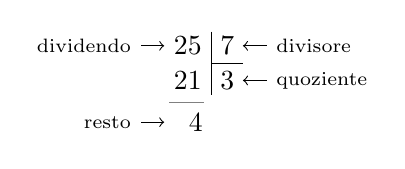
\begin{tikzpicture}

\draw[-](0,.4)--(0,-.4); % verticale
\draw[-](0,0)--(.4,0) ; %orizzontale
\draw[gray] (-.1,-.5) -- (-.54,-.5); % resto

\node (a) at (.2,.22) {7};
\node (b) at (.2,-.22) {3};
\node (c) at (-.3,.22) {25};
\node (d) at (-.3,-.22) {21};
\node (e) at (-.2,-.75){4};

\begin{scope}[font=\scriptsize]
  \draw  [<-] (.4,.22)--(.7,.22) node[right] {divisore};
  \draw  [<-] (.4,-.22)--(.7,-.22) node[right] {quoziente};
  \draw  [<-] (-.6,.22)--(-.9,.22) node[left] {dividendo};
  \draw  [<-] (-.6,-.75)--(-.9,-.75) node[left] {resto};
\end{scope}

\end{tikzpicture}

\end{center}

\end{center}
\paragraph{Passo V}
 Ripetiamo il procedimento tra il resto parziale ottenuto, $-4x^{3}+x^{2}+5x-1$ e il divisore~$3x^{2}+0x-1$. Dividiamo il primo termine del resto che
 è~$-4x^{3}$ per il primo termine del divisore che è~$3x^{2}$. Otteniamo~$-{\frac{4}{3}}x$ che è il secondo termine del quoziente.
% \newpage
\begin{center}
 \input{./lbr/chap11/fig006_div.pgf}
\end{center}
\paragraph{Passo VI}
 Proseguiamo moltiplicando~$-{\frac{4}{3}}x$ per~$B(x)$, riportiamo il risultato del prodotto, con segno opposto, sotto i
 termini del primo resto parziale e addizioniamo i due polinomi.
\begin{center}
 % (c) 2012 Dimitrios Vrettos - d.vrettos@gmail.com
\begin{tikzpicture}[font=\small]

\matrix  (a) [matrix of  nodes, anchor=south, minimum width=9mm, ,nodes={text depth=2.5mm}]{
$3x^4$&$-4x^3$&$+0x^2$&$+5x$&$-1$ &$3x^2$&$+0x$&$-1$\\
$-3x^4$&$-0x^3$&$+x^2$&&{}&$x^2$&$-\displaystyle\frac{4}{3}x$\\
{}&$-4x^3$&$+x^2$&$+5x$&$-1$\\
{}&$-4x^3$&$+0x^2$&$-\displaystyle\frac{4}{3}x$&{}\\
{}&&$x^2$&$+\displaystyle\frac{11}{3}x$&$-1$\\};

 \draw(a-1-6.north west)--(a-2-6.south west);
 \draw(a-1-6.south west)--(a-1-8.south east);
 \draw (a-2-1.south west) -- (a-2-5.south east);
\draw (a-4-2.south west) -- (a-4-5.south east);
\end{tikzpicture}
\end{center}
\paragraph{Passo VII}
 Possiamo ripetere per l'ultima volta il procedimento precedente tra il resto parziale~$R_{p}(x)=x^{2}+\frac{11}{3}x-1$ e
 il divisore~$B(x)$ in quanto hanno lo stesso grado. Dividendo il termine di grado maggiore di~$R_{p}(x)$, che è~$x^{2}$,
 per il termine di grado maggiore di~$B(x)$ che è~$3x^{2}$ si ottiene~$\frac{1}{3}$ che è il terzo termine del polinomio quoziente.
\begin{center}
 \input{./lbr/chap11/fig008_div.pgf}
\end{center}

Non possiamo più ripetere l'algoritmo poiché il resto ottenuto ha grado minore del grado del divisore.

In conclusione~$A(x):B(x)$ ha quoziente~$Q(x)=x^{2}-\dfrac{4}{3}x+\dfrac{1}{3}$ e resto~$R(x)={\dfrac{11}{3}}x-\dfrac{2}{3}$.

\paragraph{Verifica}
Verifichiamo se abbiamo svolto correttamente i calcoli; dovrebbe risultare, come detto sopra:$\quad A(x)=Q(x)\cdot B(x)+R(x)$.
\begin{equation*}
\begin{split}
\left(3x^{2}-1\right)\left(x^{2}-\frac{4}{3}x+\frac{1}{3}\right)+\frac{11}{3}x &= 3x^{4}-4x^{3}-x^{2}+\frac{4}{3}x-\frac{1}{3}+\frac{11}{3}x-\frac{2}{3}\\
                                        &= 3x^{4}-4x^{3}+\frac{15}{3}x-\frac{3}{3}\\
                                        &=x^{4}-4x^{3}+5x-1\\
                                        &=A(x).
\end{split}
\end{equation*}
I polinomi~$Q(x)$ e~$R(x)$ soddisfano quindi le nostre richieste. Ma sono unici? È sempre possibile trovarli? A queste domande risponde il seguente teorema.
 \end{esempio}
\end{exrig}

\begin{teorema}[Divisione euclidea]
 Siano~$A(x)$ e~$B(x)$ due polinomi in una sola variabile, esistono e sono unici due polinomi~$Q(x)$ e~$R(x)$, con grado di~$R(x)$
 minore o uguale del grado di~$B(x)$, tali che~$A(x)=Q(x)\cdot B(x)+R(x)$.
\end{teorema}

\osservazione Nel caso in cui il grado di~$A(x)$ sia minore del grado di~$B(x)$ il teorema resta valido, in questo caso~$Q(x)=0$ e~$R(x)=A(x)$.
Nel caso di polinomi in più variabili il teorema della divisione euclidea non vale.

\begin{definizione}
 Si dice che un polinomio~$A$ (dividendo) è \emph{divisibile} per un polinomio~$B$ (divisore)
 se esiste un polinomio~$Q$ (quoziente) per il quale~$A=Q\cdot B$.
\end{definizione}

\begin{exrig}
 \begin{esempio}
 Eseguiamo la divisione tra~$A(x)=x^{3}-2x^{2}+x-2$ e~$B(x)=x^{2}+1$.
I due polinomi sono ordinati secondo potenze decrescenti della variabile, il grado di~$A$ è maggiore del grado di~$B$ e quest'ultimo
deve essere completo. Inseriamoli nello schema per eseguire l'algoritmo. Risulta:
$\left(x^{3}-2x^{2}+x-2\right):\left(x^{2}+1\right)=(x-2)$; il resto~$R(x)$ è il polinomio nullo e~$A(x)$ è divisibile per~$B(x)$.
Infatti~$\left(x^{2}+1\right)\cdot (x-2)=\left(x^{3}-2x^{2}+x-2\right)$.
\begin{center}
 % (c) 2012 Dimitrios Vrettos - d.vrettos@gmail.com
\begin{tikzpicture}[font=\small]

\matrix  (a) [matrix of  nodes, anchor=south, minimum width=9mm,nodes={text depth=1mm}]{
$x^3$&$-2x^2$&$+x$&$-2$ &$x^2$&$+0x$&$+1$\\
$-x^3$&$-0x^2$&$-x$&{}&$x$&$-2$\\
{}&$-2x^2$&$+0x$&$-2$\\
{}&$-2x^2$&$+0x$&$-2$\\
&&&$0$&{}\\
};

\draw(a-1-5.north west)--(a-2-5.south west);
\draw(a-1-5.south west)--(a-1-7.south east);
 \draw (a-2-1.south west) -- (a-2-4.south east);
 \draw (a-4-2.south west) -- (a-4-4.south east);
\end{tikzpicture}\vspace*{-1.10ex}
\end{center}
 \end{esempio}
\end{exrig}

In conclusione, se~$A(x)$ è un polinomio di grado~$n$ e~$B(x)$ un polinomio di grado~$m$ con~$n\ge m$, quando si esegue
la divisione tra~$A$ e~$B$ si ottiene un polinomio quoziente~$Q(x)$ di grado~$n-m$ e un polinomio~$R(x)$ di grado~$g<m$.
Si dimostra che i polinomi~$Q(x)$ e~$R(x)$ sono unici.

Se~$R(x)$ è il polinomio nullo, la divisione è esatta e il polinomio~$A$ è divisibile per il polinomio~$B$.
Se~$n<m$, allora la divisione non si può eseguire e si ottiene la frazione algebrica~$\frac{A}{B}$.

\vspazio\ovalbox{\risolvii \ref{ese:11.24}, \ref{ese:11.25}, \ref{ese:11.26}, \ref{ese:11.27}, \ref{ese:11.28}}

\subsection{Polinomi in più variabili}
Per la divisione tra polinomi in più variabili riportiamo soltanto qualche esempio.
\begin{exrig}
 \begin{esempio}
Siano~$A(a\text{,~}b)=3a^{2}b+4ab^{2}+3a^{3}-2b^{3}$ e~$B(a\text{,~}b)=a-3b$ rispettivamente dividendo e divisore di una divisione tra polinomi;
essi sono due polinomi omogenei nelle due variabili~$a$ e~$b$ rispettivamente di grado~$3$ e grado~$1$.

Per eseguire la divisione procediamo come nel caso di polinomi in una sola variabile.
Dividiamo il polinomio~$A(a\text{,~}b)=3a^{2}b+4ab^{2}+3a^{3}-2b^{3}$ per il polinomio~$B(a\text{,~}b)=a-3b$ rispetto alla variabile~$a$.
Controlliamo le condizioni:
\begin{itemize*}
\item $A$ e~$B$ sono ordinati rispetto alla variabile $a$? No, $A$ non lo è. Quindi ordiniamo~$A$:
\[A(a\text{,~}b)=3a^{3}+3a^{2}b+4ab^{2}-2b^{3};\]
\item il grado di~$A$ è maggiore o uguale al grado di~$B$? Sì;
\item $A$ e~$B$ sono completi rispetto alla variabile~$a$? Sì.
\end{itemize*}
Costruiamo lo schema per eseguire l'algoritmo e procediamo:
\begin{center}
 % (c) 2012 Dimitrios Vrettos - d.vrettos@gmail.com
\begin{tikzpicture}[font=\small]

\matrix  (a) [matrix of  nodes, anchor=south, minimum width=9mm, ,nodes={text depth=2.5mm}]{
$3a^3$&$+3a^2b$&$+4ab^2$&$-2b^3$&$a$&$-3b$\\
{}&{}&$\ldots$&{}&$3a^2$&-\ldots\\
};

\draw(a-1-5.north west)--(a-2-5.south west);
\draw(a-1-5.south west)--(a-1-6.south east);
\end{tikzpicture}
\end{center}
Il quoziente è~$Q =\ldots \ldots \ldots$; il resto~$R = 118b^{3}$

Verifica~$\ldots \ldots \ldots \ldots \ldots \ldots$

Se avessimo eseguito la divisione rispetto alla variabile~$b$, avremmo ottenuto stesso quoziente e stesso resto? Proviamo.
Controlliamo le condizioni:
\begin{itemize*}
\item $A$ e~$B$ sono ordinati rispetto alla variabile~$b$? No. Ordinando~$A$, risulta:
\[A(a\text{,~}b)=-2b^{3}+4ab^{2}+3a^{2}b+3a^{3}+3a^{2}b;\]
e ordinando~$B$, risulta
\[B(a\text{,~}b)=-3b+a;\]
\item il grado di~$A$ è maggiore o uguale al grado di~$B$? Sì;
\item $A$ e~$B$ sono completi rispetto alla variabile~$b$? Sì.
\end{itemize*}
Costruisci lo schema dell'algoritmo e concludi.
 \end{esempio}
\end{exrig}
\ovalbox{\risolvii \ref{ese:11.29}, \ref{ese:11.30}}

\section{Regola di Ruffini}\label{sect:regola_di_Ruffini}

Per eseguire la divisione tra due polinomi in una sola variabile, \emph{nel caso in cui il
divisore sia di grado~1} si può applicare una regola nota come \emph{regola
di Ruffini}\footnote{dal nome del matematico e medico italiano Paolo Ruffini (1765 - 1822).} (o \emph{divisione sintetica}) e che si basa sui seguenti teoremi.

\begin{teorema}
 Il resto della divisione di un polinomio~$A(x)$ per un
binomio del tipo~$(x-k)$ è uguale al valore che~$A(x)$ assume quando
al posto della variabile $x$ si sostituisce il valore $k$, $R=A(k)$.
\end{teorema}

\begin{proof}
 Dalla divisione di~$A(x)$ per~$x-k$ otteniamo la seguente
uguaglianza:
\[A(x)=(x-k)\cdot Q(x)+R\]
in cui si è scritto~$R$ anziché $R(x)$, poiché è
una costante.

Essendo tale relazione valida per qualsiasi valore che si attribuisce
alla variabile~$x$, sostituiamo al suo posto il valore
$k$ e otteniamo:

\[A(k)=\underbrace{(k-k)}_{0}\cdot Q(k)+R=R.\]

Ciò vuol dire che il valore assunto da~$A(x)$
quando~$x=k$ è proprio uguale al resto della divisione.
\end{proof}

\begin{teorema}[di Ruffini]
 Condizione necessaria e sufficiente affinché un
polinomio~$A(x)$ sia divisibile per un binomio del tipo~$(x-k)$ è
che risulti~$A(k)=0$.
\end{teorema}

\begin{proof}
\emph{Prima implicazione}:~$A(x)$ divisibile per~$(x-k)\:\Rightarrow\: A(k)=0$.

Poiché $A(x)$ è divisibile per~$(x-k)$, per definizione di divisibilità deve essere~$R=0$. Ma, per il
teorema del resto, $A(k)=R=0$, quindi, per la proprietà transitiva
dell'uguaglianza, $A(k)=0$.

\emph{Seconda implicazione}:~$A(k)=0\:\Rightarrow\: A(x)$
divisibile per~$(x-k)$.

Il resto della divisione del polinomio~$A(x)$ per il binomio~$x-k$,
per il teorema del resto risulta~$R=A(k)$ e per ipotesi~$A(k)=0$,
ne segue che~$R=0$. Per definizione di divisibilità, essendo il
resto della divisione zero, segue che~$A(x)$ è divisibile per~$(x-k)$.
\end{proof}


\begin{procedura}
 Dividere un polinomio con la regola di Ruffini:

 \begin{enumeratea}
 \item calcolo del resto;
\item applicazione del procedimento di divisione;
\item verifica.
 \end{enumeratea}
\end{procedura}


\begin{exrig}
 \begin{esempio}
$\left(a^{2}-3a+1\right):(a-1).$

Dividiamo con la regola di Ruffini il polinomio~$A(a)=a^{2}-3a+1$ per
il binomio~$B(a)=a-1$; cerchiamo quoziente~$Q(a)$ e resto~$R(a)$.

\paragraph{Passo I} \emph{Calcolo del polinomio resto.}

Si considera il termine numerico del polinomio divisore cambiato di
segno (nell'esempio è~1) e si sostituisce alla
lettera del polinomio dividendo~$A(1)$:~$1^{2}-3\cdot 1 + 1 = 1 - 3 + 1 = -1$.

Il resto della divisione è~$-1$.

\paragraph{Passo II} \emph{Applicazione del procedimento di divisione.}

Disegnare il seguente schema di Ruffini: scrivere i coefficienti
numerici del polinomio dividendo, secondo le potenze decrescenti della
variabile. Se manca un termine occorre mettere~0.
L'ultimo termine numerico è messo esternamente alla
griglia. Nell'angolo a sinistra dello schema si pone il
termine numerico del polinomio divisore cambiato di segno,
nell'esempio è~1.

\begin{center}
% (c) 2012 Dimitrios Vrettos - d.vrettos@gmail.com
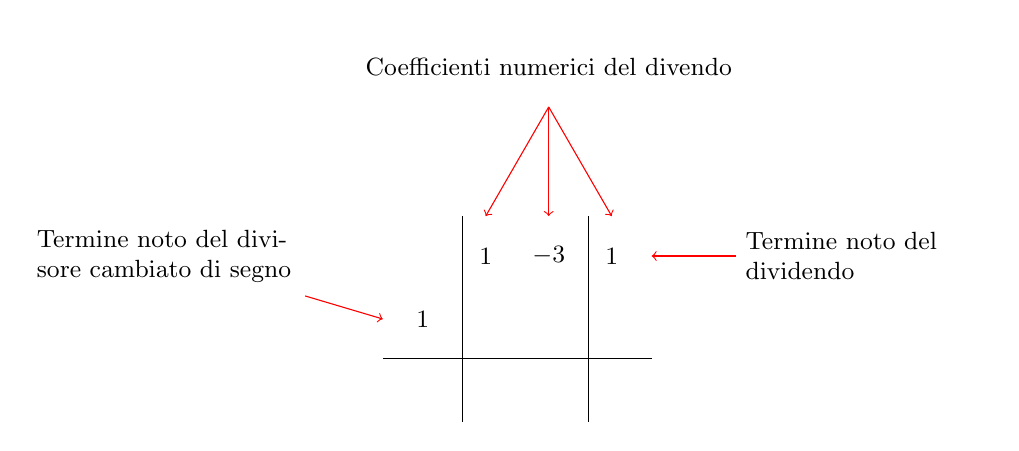
\begin{tikzpicture}[font=\small,x=8mm, y=8mm, minimum size=10mm]

\node (a0) at (0,0) {};
\node (a1) at (1,0) {1};
\node (a2) at (2,0) {$-3$};
\node (a3) at (3,0) {1};

\node(a4) at (0,-1) {1};
\node (a5) at (1,-1) {};
\node (a6) at (2,-1) {};
\node (a7) at (3,-1) {};

\node (a8) at (0,-2) {};
\node (a9) at (1,-2) {};
\node (a10) at (2,-2) {};
\node (a11) at (3,-2) {};

\draw (a0.north east)--(a8.south east);
 \draw (a4.south west)--(a7.south east);
\draw (a2.north east)--(a10.south east);

\node (b) at (2,3) {Coefficienti numerici del divendo};
\node[text width=3.4cm] (c) at (-4,0){Termine noto del divisore cambiato di segno};
\node[text width=3cm] (d) at (7,0) {Termine noto del dividendo};

\begin{scope}[->, red]
\foreach \x in {a1.north, a2.north, a3.north}
	\draw (b.south)--(\x);
\draw (c) -- (a4.west);
\draw (d)-- (a3.east);
\end{scope}

\end{tikzpicture}
\end{center}

\begin{multicols}{2}
 Il primo termine si riporta inalterato nella parte sottostante:
\begin{center}
\input{./lbr/chap11/fig013_ruf.pgf}
\end{center}
\end{multicols}

\begin{multicols}{2}
 Moltiplicare il termine noto del divisore (cambiato di segno) per il
primo coefficiente appena trascritto e riportare il risultato sotto il
secondo coefficiente
\begin{center}
\input{./lbr/chap11/fig014_ruf.pgf}
\end{center}
\end{multicols}

\begin{multicols}{2}
 Sommare i due termini appena incolonnati~$-3+1=-2$.
\begin{center}
\input{./lbr/chap11/fig015_ruf.pgf}
\end{center}
\end{multicols}

\begin{multicols}{2}
 Moltiplicare il termine noto del divisore (cambiato di segno) per la
somma appena ottenuta~$1\cdot (-2)=-2$.
\begin{center}
% (c) 2012 Dimitrios Vrettos - d.vrettos@gmail.com
\begin{tikzpicture}[font=\small,x=8mm, y=8mm, minimum size=10mm]

\node (a0) at (0,0) {};
\node (a1) at (1,0) {1};
\node (a2) at (2,0) {$-3$};
\node (a3) at (3,0) {1};

\node(a4) at (0,-1) {1};
\node (a5) at (1,-1) {};
\node (a6) at (2,-1) {1};
\node (a7) at (3,-1) {$-2$};

\node (a8) at (0,-2) {};
\node (a9) at (1,-2) {1};
\node (a10) at (2,-2) {$-2$};
\node (a11) at (3,-2) {};

\draw (a0.north east)--(a8.south east);
 \draw (a4.south west)--(a7.south east);
\draw (a2.north east)--(a10.south east);

\begin{scope}[->,red]
\draw (a4.east)--(a10.west);
\draw (a10.east)--(a7.south);
\end{scope}
\end{tikzpicture}

\end{center}
\end{multicols}
%\newpage
\begin{multicols}{2}
 Addizionare gli ultimi due numeri incolonnati~$1-2=-1$.
\begin{center}
% (c) 2012 Dimitrios Vrettos - d.vrettos@gmail.com
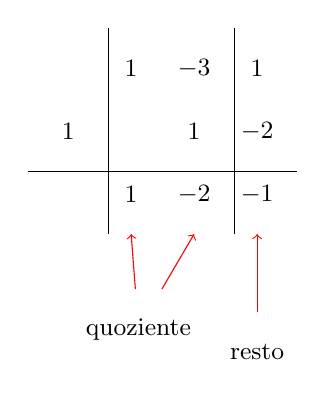
\begin{tikzpicture}[font=\small,x=8mm, y=8mm, minimum size=10mm]

\node (a0) at (0,0) {};
\node (a1) at (1,0) {1};
\node (a2) at (2,0) {$-3$};
\node (a3) at (3,0) {1};

\node(a4) at (0,-1) {1};
\node (a5) at (1,-1) {};
\node (a6) at (2,-1) {1};
\node (a7) at (3,-1) {$-2$};

\node (a8) at (0,-2) {};
\node (a9) at (1,-2) {1};
\node (a10) at (2,-2) {$-2$};
\node (a11) at (3,-2) {$-1$};

\draw (a0.north east)--(a8.south east);
 \draw (a4.south west)--(a7.south east);
\draw (a2.north east)--(a10.south east);

\node[below left of=a10,below=5mm](q)  {quoziente};
\node[below of=a11, below=5mm](r)  {resto};
\begin{scope}[->,red]
\draw (q)--(a9.south);
\draw (q)--(a10.south);
\draw (r)--(a11.south);
\end{scope}
\end{tikzpicture}
\end{center}
\end{multicols}

Infine si ricostruisce il polinomio quoziente, tenendo presente che i
coefficienti numerici sono quelli trovati da questa divisione, cioè~1
e~$-2$. Quoziente e resto sono allora~$Q(x)=a-2$ e~$R=-1$.

\paragraph{Passo III}\emph{Verifica}

Come nella divisione con i numeri, si moltiplica il polinomio risultato
per il polinomio divisore e si somma il polinomio resto. Il risultato
deve essere il polinomio dividendo.
\[(a - 2)(a - 1) + (-1) = a^{2} - a - 2a + 2 - 1 =a^{2}-3a + 1.\]
 \end{esempio}

\begin{esempio}
$(4x^{3} - 5x + 6): (x + 1).$

Applicazione del procedimento di divisione
\begin{center}
% (c) 2012 Dimitrios Vrettos - d.vrettos@gmail.com
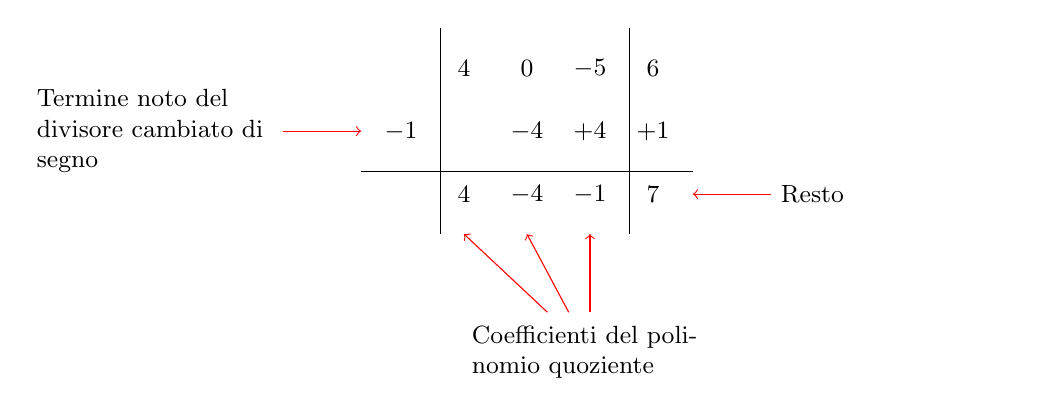
\begin{tikzpicture}[font=\small,x=8mm, y=8mm, minimum size=10mm]

\node (a0) at (0,0) {};
\node (a1) at (1,0) {4};
\node (a2) at (2,0) {0};
\node (a3) at (3,0) {$-5$};
\node (a4) at (4,0) {6};

\node(a5) at (0,-1) {$-1$};
\node (a6) at (1,-1) {};
\node (a7) at (2,-1) {$-4$};
\node (a8) at (3,-1) {$+4$};
\node (a9) at (4,-1) {$+1$};

\node (a10) at (0,-2) {};
\node (a11) at (1,-2) {4};
\node (a12) at (2,-2) {$-4$};
\node (a13) at (3,-2) {$-1$};
\node (a14) at (4,-2) {7};

\draw (a0.north east)--(a10.south east);
 \draw (a5.south west)--(a9.south east);
\draw (a3.north east)--(a13.south east);

 \node[text width=3cm, left of=a5, left=5mm](b)  {Termine noto del divisore cambiato di segno};
 \node[text width=3cm, below of=a13, below=5mm](c)  {Coefficienti del polinomio quoziente};
 \node[text width=3cm, right of=a14, right=5mm](d)  {Resto};
 \begin{scope}[->,red]
 \draw (b)--(a5.west);
 \draw (d)--(a14);
\foreach \x in {a11,a12,a13}
\draw (c)--(\x.south);
 \end{scope}
\end{tikzpicture}
\end{center}
\[Q(x)=4x^{2}-4x-1 \qquad R=7.\]
\end{esempio}

\textit{Verifica.}

\[Q(x)\cdot B(x)+R=A(x)\]

\[\left(4x^{2}-4x-1\right)\cdot (x+1)+7=4x^{3}+4x^{2}-4x-x-1+7=4x^{3}-5x+6\]

Vediamo il caso in cui il binomio che fa da divisore ha coefficiente
numerico della variabile diverso da~1.


\begin{esempio}
 Dividere con la regola di Ruffini~$\left(2x^{4}-x^{3}-4x^{2}+2x+7\right):(2x-1)$.

In questo tipo di esercizi si deve rendere il divisore del tipo~$x+n$,
quindi nel nostro caso si deve dividere sia il dividendo sia il
divisore per~2; sappiamo, infatti, dalla proprietà invariantiva della
divisione che dividendo per uno stesso numero dividendo e divisore il
quoziente della divisione non cambia. Il resto invece risulterà
diviso per~2. Quindi applichiamo l'algoritmo precedente
e \emph{ricordiamoci al termine della divisione di moltiplicare il
resto per}~2.

La divisione allora diventa
$\left(x^{4}-\frac{1}{2}x^{3}-2x^{2}+x+\frac{7}{2}\right):\left(x-\frac{1}{2}\right)$.
\end{esempio}
\end{exrig}

\ovalbox{\risolvii \ref{ese:11.31}, \ref{ese:11.32}, \ref{ese:11.33}, \ref{ese:11.34}, \ref{ese:11.35}}

\subsection{Calcolo del resto}

Si considera il termine numerico del polinomio divisore cambiato di
segno (nell'esempio precedente è~$+{\frac{1}{2}}$) e si
sostituisce alla lettera che compare nel polinomio dividendo. Il risultato che si
ottiene è il resto della
divisione~$\left(\frac{1}{2}\right)^{4}-\frac{1}{2}\left(\frac{1}{2}\right)^{3}-2\left(\frac{1}{2}\right)^{2}+\frac{1}{2}+\frac{7}{2}=-\frac{1}{16}-\frac{1}{2}+\frac{1}{2}+\frac{7}{2}=\frac{7}{2}$.

Applicazione del procedimento di divisione.
\begin{center}
 % (c) 2012 Dimitrios Vrettos - d.vrettos@gmail.com
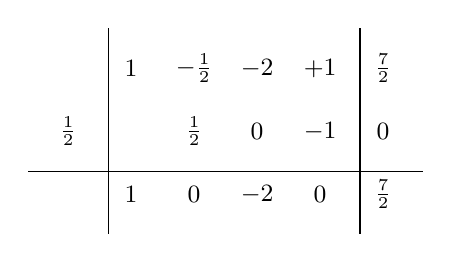
\begin{tikzpicture}[font=\small,x=8mm, y=8mm, minimum size=10mm]

\node (a0) at (0,0) {};
\node (a1) at (1,0) {1};
\node (a2) at (2,0) {$-\frac{1}{2}$};
\node (a3) at (3,0) {$-2$};
\node (a4) at (4,0) {$+1$};
\node (a5) at (5,0) {$\frac{7}{2}$};

\node(a6) at (0,-1) {$\frac{1}{2}$};
\node (a7) at (1,-1) {};
\node (a8) at (2,-1) {$\frac{1}{2}$};
\node (a9) at (3,-1) {0};
\node (a10) at (4,-1) {$-1$};
\node (a11) at (5,-1) {0};

\node (a12) at (0,-2) {};
\node (a13) at (1,-2) {1};
\node (a14) at (2,-2) {0};
\node (a15) at (3,-2) {$-2$};
\node (a16) at (4,-2) {0};
\node (a17) at (5,-2) {$\frac{7}{2}$};

\draw (a0.north east)--(a12.south east);
 \draw (a6.south west)--(a11.south east);
\draw (a4.north east)--(a16.south east);

\end{tikzpicture}
\end{center}

Adesso si pone la lettera per ogni termine del polinomio risultato
partendo dal grado del polinomio dividendo diminuito di~1. Il risultato
è quindi il polinomio~$x^{3}-2x$, il resto è~$\frac{7}{2}\cdot2=7$.

\paragraph{Verifica}
Per la proprietà della divisione si moltiplica il quoziente per il
polinomio divisore e si somma il resto ottenuto. Il risultato deve
essere il polinomio dividendo.

\[\left(x^{3}-2x\right)(2x-1)+7=2x^{4}-x^{3}-4x^{2}+2x+7.\]

In generale, se si vuole dividere il polinomio~$A(x)$ per il binomio~$(nx-\alpha)$, utilizzando la proprietà invariantiva della
divisione, si divide dividendo e divisore per~$n$, così da ottenere un divisore con coefficiente 1 per il termine di primo grado. Quindi si può effettuare la divisione ottenendo il quoziente $Q(x)$ ed il resto $R$. Per ottenere il resto della divisione di
partenza occorre moltiplicare $R$ per il coefficiente~$n$.
Infatti si ha:~$A(x)=(nx-\alpha)Q(x)+R $
e, dividendo ambo i membri per~$n$, si ha:
\[\frac{A(x)}{n}=\left(x-\frac{\alpha }{n}\right)Q(x)+\frac{R}{n}.\]
\ovalbox{\risolvii \ref{ese:11.36}, \ref{ese:11.37}, \ref{ese:11.38}, \ref{ese:11.39}, \ref{ese:11.40}, \ref{ese:11.41}}
\newpage
% (c) 2012-2014 Dimitrios Vrettos - d.vrettos@gmail.com
% (c) 2012, 2014 Claudio Carboncini - claudio.carboncini@gmail.com
% (c) 2012 Silvia Cibola - silvia.cibola@gmail.com
\section{Esercizi}
\subsection{Esercizi dei singoli paragrafi}
\subsubsection*{11.1 - Definizioni fondamentali}
\begin{multicols}{2}
\begin{esercizio}
\label{ese:11.1}
Riduci in forma normale il seguente polinomio:
\[5a^3-4ab-1+2a^3+2ab-a-3a^3.\]
\emph{Svolgimento}: Evidenziamo i termini simili e sommiamoli tra di loro:
\[\underline{5a^3}-\overline{4ab}+1+\underline{2a^3}+\overline{2ab}-a-\underline{3a^3}.\]
%\[\mmevid{ev_rosso}{5a^{3}}-\mmevid{ev_verde}{4ab}+1+\mmevid{ev_rosso}{2a^{3}}+\mmevid{ev_verde}{2ab}-a-\mmevid{ev_rosso}{3a^{3}}\]
%così otteniamo \dotfill Il termine noto è \dotfill
\end{esercizio}

\begin{esercizio}
\label{ese:11.2}
Il grado di:
\begin{enumeratea}
\item $x^2y^2−3y^3+5yx−6y^2x^3$ rispetto alla lettera~$y$ è \dotfill, il grado complessivo è \dotfill
\item $5a^2−b+4ab$ rispetto alla~$b$ è \dotfill,\\ il grado complessivo è \dotfill
\end{enumeratea}
\end{esercizio}


\begin{esercizio}
\label{ese:11.3}
Quali polinomi sono omogenei:
\begin{enumeratea}
\item $x^3y+2y^2x^2−4x^4$;
\item $2x+3−xy$;
\item $2x^3y^3−y^4x^2+5x^6$.
\end{enumeratea}
\end{esercizio}

\begin{esercizio}
\label{ese:11.4}
Quali dei seguenti polinomi sono ordinati rispetto alla lettera~$x$ con potenze crescenti:

\begin{enumeratea}
\item $2-\dfrac{1}{2}x^2+x$;
\item $\dfrac{2}{3}-x+3x^2+5x^3$;
\item $3x^4-\dfrac{1}{2}x^3+2x^2-x+\dfrac{7}{8}$.
\end{enumeratea}
\end{esercizio}

\begin{esercizio}
\label{ese:11.5}
Relativamente al polinomio~$b^2+a^4+a^3+a^2$ Il grado massimo è \ldots il grado rispetto alla lettera~$a$ è \ldots 

Rispetto alla lettera~$b$ è \ldots\, Il polinomio è ordinato rispetto alla $a$? È completo? È omogeneo?
%\begin{itemize*}
%\item Il grado massimo è \ldots. Il grado rispetto alla lettera~$a$ è \ldots. Rispetto alla lettera~$b$ è \ldots
%\item il polinomio è ordinato rispetto alla $a$? %\tab\qquad\boxV\qquad\boxF
%\item è completo? %\tab\qquad\boxV\qquad\boxF
%\item è omogeneo? %\tab\qquad\boxV\qquad\boxF
%\end{itemize*}
\end{esercizio}

\begin{esercizio}
\label{ese:11.6}
Scrivi un polinomio di terzo grado nelle variabili~$a$ e~$b$ che sia omogeneo.
\end{esercizio}

\begin{esercizio}
\label{ese:11.7}
Scrivi un polinomio di quarto grado nelle variabili~$x$ e~$y$ che sia omogeneo e ordinato secondo le
potenze decrescenti della seconda indeterminata.
\end{esercizio}

\begin{esercizio}
\label{ese:11.8}
Scrivi un polinomio di quinto grado nelle variabili~$r$ e~$s$ che sia omogeneo e ordinato secondo le
potenze crescenti della prima indeterminata.
\end{esercizio}

\begin{esercizio}
\label{ese:11.9}
Scrivi un polinomio di quarto grado nelle variabili~$z$ e~$w$ che sia omogeneo e ordinato secondo le
potenze crescenti della prima indeterminata e decrescenti della seconda.
\end{esercizio}

\begin{esercizio}
\label{ese:11.10}
Scrivi un polinomio di sesto grado nelle variabili~$x$, $y$ e~$z$ che sia completo e ordinato secondo le
potenze decrescenti della seconda variabile.
\end{esercizio}


\begin{esercizio}
\label{ese:11.11}
Calcola il valore numerico dei polinomi per i valori a fianco indicati.

\begin{enumeratea}
\item $x^2+x$ per $x=-1$;
\item $2x^2-3x+1$ per $x=0$;
\item $3x^2-2x-1$ per $x=2$;
\item $3x^3-2x+x$ per $x=-2$;
\item $\dfrac{3}{4}a+\dfrac{1}{2}b-\dfrac{1}{6}ab$ per $a=-\dfrac{1}{2}$, $b=3$;
\item $4x-6y+\dfrac{1}{5}x^2$ per $x=-5$, $y=\dfrac{1}{2}$.
\end{enumeratea}
\end{esercizio}
\end{multicols}


\subsubsection*{11.2 - Somma algebrica di polinomi}
\begin{esercizio}
\label{ese:11.12}
Calcolare la somma dei due polinomi:~$2x^2+5−3y^2x$, $x^2−xy+2−y^2x+y^3$.

\emph{Svolgimento}: Indichiamo la somma~$(2x^2+5−3y^2x)+(x^2−xy+2−y^2x+y^3)$, eliminando le parentesi otteniamo
il polinomio~$2x^2+5−3y^2x+x^2−xy+2−y^2x+y^3$, sommando i monomi simili otteniamo~$3x^2−4x^{\ldots}y^{\ldots}-\ldots xy+y^3+\ldots$
\end{esercizio}
%\newpage
\begin{esercizio}
\label{ese:11.13}
 Esegui le seguenti somme di polinomi.
\begin{multicols}{3}
 \begin{enumeratea}
 \item $a+b-b$;
 \item $a+b-2b$;
 \item $a+b-(-2b)$;
 \item $a-(b-2b)$;
 \item $2a+b+(3a+b)$;
 \item $2a+2b+(2a+b)+2a$;
 \item $2a+b-(-3a-b)$;
 \item $2a-3b-(-3b-2a)$;
 \item $(a+1)-(a-3)$.
\end{enumeratea}
\end{multicols}
\end{esercizio}

\begin{esercizio}[\Ast]
\label{ese:11.14}
 Esegui le seguenti somme di polinomi.

 \begin{enumeratea}
 \item $\left(2a^{2}-3b\right)+\left(4b+3a^{2}\right)+\left(a^{2}-2b\right)$;
 \item $\left(3a^{3}-3b^{2}\right)+\left(6a^{3}+b^{2}\right)+\left(a^{3}-b^{2}\right)$;
 \item $\left(\dfrac{1}{5}x^{3}-5x^{2}+\dfrac{1}{5}x-1\right)-\left(3x^{3}-\dfrac{7}{3}x^{2}+\dfrac{1}{4}x-1\right)$;
 \item $\left(\dfrac{1}{2}+2a^{2}+x\right)-\left(\dfrac{2}{5}a^{2}+\dfrac{1}{2}{ax}\right)+\left[-\left(-{\dfrac{3}{2}}-2{ax}+x^{2}\right)+\dfrac{1}{3}a^{2}\right]-\left(\dfrac{3}{2}{ax}+2\right)$;
 \item $\left(\dfrac{3}{4}a+\dfrac{1}{2}b-\dfrac{1}{6}{ab}\right)-\left(\dfrac{9}{8}{ab}+\dfrac{1}{2}a^{2}-2b\right)+{ab}-\dfrac{3}{4}a$.
\end{enumeratea}
\end{esercizio}

\begin{esercizio}[\Ast]
\label{ese:11.15} %nuovo
 Esegui le seguenti somme di polinomi.

 \begin{enumeratea}
 \item $\left(a+b^{2}+c^{3}\right)+\left(-4a-5c^{3}\right)+\left(8a-7b^{2}+10c^{3}\right)+\left(6b^{2}-7c^{3}\right)$;
 \item $\left(\dfrac{3}{2}x^{2}-\dfrac{5}{3}xy+2y^{2}\right)+\left(\dfrac{3}{4}x^{2}+\dfrac{1}{5}xy-\dfrac{4}{3}y^{2}\right)$;
 \item $\left(\dfrac{1}{2}x^{2}-2x+3\right)+\left(\dfrac{3}{2}x^{2}-x+\dfrac{1}{3}\right)+\left(\dfrac{2}{3}x^{2}-\dfrac{1}{2}x+\dfrac{2}{3}\right)+\left(\dfrac{7}{5}x^{2}-2+\dfrac{3}{4}x\right)$;
 \item $\left(2a^{3}-\dfrac{1}{4}\right)+\left(-3a^{3}-\dfrac{2}{5}a^{2}+\dfrac{3}{4}\right)+\left(\dfrac{2}{5}a^{2}-\dfrac{1}{2}a+\dfrac{1}{4}a^{3}\right)$;
 \item $\left(x^{4}-\dfrac{1}{2}x^{2}+2x^{3}-\dfrac{1}{3}x\right)+\left(-\dfrac{2}{5}x^{4}-\dfrac{2}{3}x^{3}+\dfrac{5}{3}x^{2}+x-1\right)+\left(2x^{2}-1-\dfrac{4}{3}x^{3}-\dfrac{2}{3}x\right)-\dfrac{1}{6}x^2$.
\end{enumeratea}
\end{esercizio}

\begin{esercizio}[\Ast]
\label{ese:11.16} %nuovo
 Esegui le seguenti somme di polinomi.

 \begin{enumeratea}
 \item $(2ab-3)+\left(a^{2}b-2ab\right)-\left(4+a^{2}b\right)$;
 \item $\dfrac{2ab+3}{2}-\dfrac{4a+b-5}{3}+3ab-\dfrac{19+8a-2b}{6}$;
 \item $(3a-2+b)-\left(\dfrac{4}{3}+\dfrac{a}{2}-\dfrac{b}{3}\right)-\dfrac{9a+2b-20}{6}$;
 \item $\dfrac{4-3ab}{2}-\dfrac{3+4ab}{4}-\dfrac{10ab-5}{4}$;
 \item $\left(2a^{2}b-7ab+{3}\right)-\left(a^{2}b-6ab-3\right)+\left(3ab+3a^{2}b\right)$;
 \item $\dfrac{7ab-3a^{2}+b^{2}}{3}-\left(2b^{2}-a^{2}+2ab\right)+\dfrac{b^{2}}{3}$.
\end{enumeratea}
\end{esercizio}

\begin{esercizio}[\Ast]
\label{ese:11.17} %nuovo
 Esegui le seguenti somme di polinomi.

 \begin{enumeratea}
 \item $5y+3x-[7x-3y-(5x-7y)]+(x-y)-(x-y)$;
 \item $\left(3-\dfrac{1}{2}x-2x^{2}\right)-\left(4x^{2}+\dfrac{1}{2}x+3x^{4}-2\right)+\left(1+3x^{2}-3x\right)-\left(-5x-5x^{2}+6+x^{4}\right)$;
 \item $\left(a^{3}-4a^{2}b+6ab^{3}-b^{3}\right)-\left(a^{3}-b^{3}-4a^{2}b+3ab^{3}\right)$;
 \item $\left[7a-\left(a^{2}-2\right)\right]+\left\lbrace 3a^{2}-4a+\left[6a^{2}-(2a-10)\right]-2 \right\rbrace$;
 \item $\left(b-\dfrac{a}{18}\right)-\left(\dfrac{7b}{8}-\dfrac{a}{6}\right)-\left(\dfrac{3}{4}b-\dfrac{5}{9}a\right)$.
\end{enumeratea}
\end{esercizio}

\subsubsection*{11.3 - Prodotto di un polinomio per un monomio}

\begin{esercizio}
\label{ese:11.18} %{ese:11.15}
 Esegui i seguenti prodotti di un monomio per un polinomio.
 \begin{multicols}{3}
\begin{enumeratea}
 \item $(a + b)b$;
 \item $(a - b)b$;
 \item $(a +b)(-b)$;
 \item $(a - b + 51)b$;
 \item $(-a - b -51)(-b)$;
 \item $(a^{2} - a)a$;
 \item $(a^{2} - a)(-a)$;
 \item $(a^{2}- a - 1)a^{2}$;
 \item $(a^{2}b-ab - 1)(ab)$;
 \item $(ab- ab - 1)(ab)$;
 \item $(a^{2}b- ab -1)(a^{2}b^{2})$;
 \item $(a^{2}b-ab - 1)(ab)^{2}$;
 \item $ab(a^{2}b- ab -1)ab$;
 \item $-2a(a^{2} - a - 1)(-a^{2})$;
 \item $(x^{2}a- ax+2)(2x^{2}a^{3})$.
\end{enumeratea}
\end{multicols}
\end{esercizio}

\begin{esercizio}
\label{ese:11.19} %{ese:11.16}
 Esegui i seguenti prodotti di un monomio per un polinomio.
 \begin{multicols}{2}
\begin{enumeratea}
 \item $\dfrac{3}{4}x^{2}y\cdot\left(2{xy}+\dfrac{1}{3}x^{3}y^{2}\right)$;
 \item $\left(\dfrac{a^{4}}{4}+\dfrac{a^{3}}{8}+\dfrac{a^{2}}{2}\right)\left(2a^{2}\right)$;
 \item $\left(\dfrac{1}{2}a-3+a^{2}\right)\left(-{\dfrac{1}{2}}a\right)$;
 \item $\left(5x+3{xy}+\dfrac{1}{2}y^{2}\right)\left(3x^{2}y\right)$;
 \item $\left(\dfrac{2}{3}xy^{2}+\dfrac{1}{2}x^{3}-\dfrac{3}{4}{xy}\right)(6{xy})$;
 \item $-\dfrac{1}{3}y\left(6x^{2}y-3{xy}\right)$;
 \item $-3xy^2\left(\dfrac{1}{3}x+1\right)$;
 \item $\left(\dfrac{7}{3}b-b\right)\left(a-\dfrac{1}{2}b+1\right)(3a-2a)$.
\end{enumeratea}
\end{multicols}
\end{esercizio}
%\newpage
\subsubsection*{11.4 - Quoziente tra un polinomio e un monomio}
\begin{esercizio}
\label{ese:11.20} %{ese:11.17}
 Svolgi le seguenti divisioni tra polinomi e monomi.
 \begin{multicols}{2}
\begin{enumeratea}
 \item $\left(2x^{2}y+8{xy}^{2}\right):\left(2{xy}\right)$;
 \item $\left(a^{2}+a\right):a$;
 \item $\left(a^{2}-a\right):(-a)$;
 \item $\left(\dfrac{1}{2}a-\dfrac{1}{4}\right):\dfrac{1}{2}$;
 \item $\left(\dfrac{1}{2}a-\dfrac{1}{4}\right):2$;
 \item $(2a-2):\dfrac{1}{2}$;
 \item $\left(\dfrac{1}{2}a-\dfrac{a^{2}}{4}\right):\dfrac{a}{2}$.
\end{enumeratea}
\end{multicols}
\end{esercizio}

\begin{esercizio}
\label{ese:11.21} %{ese:11.18}
 Svolgi le seguenti divisioni tra polinomi e monomi.
 \begin{multicols}{2}
\begin{enumeratea}
 \item $\left(a^{2}-a\right):a$;
 \item $\left(a^{3}+a^{2}-a\right):a$;
 \item $\left(8a^{3}+4a^{2}-2a\right):2a$;
 \item $\left(a^{3}b^{2}+a^{2}b-ab\right):b$;
 \item $\left(a^{3}b^{2}-a^{2}b^{3}-ab^{4}\right):(-{ab}^{2})$;
 \item $\left(a^{3}b^{2}+a^{2}b-ab\right):ab$;
 \item $\left(16x^{4}-12x^{3}+24x^{2}\right):\left(4x^{2}\right)$.
 \item $\left(-x^{3}+3x^{2}-10x+5\right):(-5)$;
\end{enumeratea}
\end{multicols}
\end{esercizio}

\begin{esercizio}
\label{ese:11.22} %{ese:11.19}
 Svolgi le seguenti divisioni tra polinomi e monomi.

\begin{enumeratea}
 \item $\left[\left(-3a^{2}b^{3}-2a^{2}b^{2}+6a^{3}b^{2}\right):(-3{ab})\right]\cdot\left(\dfrac{1}{2}b^{2}\right)$;
 \item $\left(\dfrac{4}{3}a^{2}b^{3}-\dfrac{3}{4}a^{3}b^{2}\right):\left(-{\dfrac{3}{2}a^{2}b^{2}}\right)$;
 \item $\left(2a+\dfrac{a^{2}}{2}-\dfrac{a^{3}}{4}\right):\left(\dfrac{a}{2}\right)$;
 \item $\left(\dfrac{1}{2}a-\dfrac{a^{2}}{4}-\dfrac{a^{3}}{8}\right):\left(\dfrac{1}{2}a\right)$;
 \item $\left(-4x^{3}+\dfrac{1}{2}x^{2}\right):\left(2x^{2}-3x^{2}+\dfrac{1}{2}x^{2}\right)$;
 \item $\left(a^{3}b^{2}-a^{4}b+a^{2}b^{3}\right):\left(a^{2}b\right)$;
 \item $\left(a^{2}-a^{4}+a^{3}\right):\left(a^{2}\right)$.
\end{enumeratea}
\end{esercizio}

\subsubsection*{11.5 - Prodotto di polinomi}
\begin{esercizio}
\label{ese:11.23} %{ese:11.20}
Esegui i seguenti prodotti di polinomi.
\begin{multicols}{2}
\begin{enumeratea}
 \item $\left(\dfrac{1}{2}a^{2}b-2{ab}^{2}+\dfrac{3}{4}a^{3}b\right)\cdot\left(\dfrac{1}{2}{ab}+b\right)$;
 \item $\left(x^{3}-x^{2}+x-1\right)({x}-1)$;
 \item $\left(a^{2}+2{ab}+b^{2}\right)(a+b)$;
 \item $(a-1)(a-2)(a-3)$;
 \item $(a+1)(2a-1)(3a-1)$;
 \item $(a+1)\left(a^{2}+a\right)\left(a^{3}-a^{2}\right)$.
\end{enumeratea}
\end{multicols}
\end{esercizio}

\subsubsection*{11.6 - Divisioni tra due polinomi}

\begin{esercizio}
\label{ese:11.24}
Completa la divisione
\begin{center}
 % (c) 2012 Dimitrios Vrettos - d.vrettos@gmail.com
\begin{tikzpicture}[x=10mm, y=10mm]

\begin{scope}[->]
\draw (-.5,0) -- (12,0);
\draw (0,-.5) -- (0,7);
\end{scope}

\foreach \x in {1,2,...,11}
\draw (\x,1.5pt) -- (\x,-1.5pt);

\foreach \y in {1,2,...,6}
\draw (1.5pt,\y) -- (-1.5pt,\y);

\foreach \xi/\xtext in {1/A,2/B,3/C,4/D,5/E,6/F,7/G,8/H,9/I,10/L,11/M}
\node[below] at (\xi,0) {$\xtext$};

\foreach \yi/\ytext in {1/1,2/2,3/3,4/4,5/5,6/6}
\node[left] at (0,\yi){\ytext};

\draw[orange, dotted] (0,0) grid (11,6);

\begin{scope}[fill=CornflowerBlue]
\foreach \x in {1,6}
\filldraw (\x,1) circle (2pt);

\foreach \x in {2,5,8}
\filldraw (\x,2) circle (2pt);

\foreach \x in {4,10}
\filldraw (\x,4) circle (2pt);

\filldraw (3,5) circle (2pt);
\filldraw (11,6) circle (2pt);
\end{scope}
\end{tikzpicture}
\end{center}
\end{esercizio}

\begin{esercizio}[\Ast]
\label{ese:11.25}
Esegui le divisioni tra polinomi.
\begin{multicols}{2}
 \begin{enumeratea}
 \item $\left(3x^{2}-5x+4\right):\left(2x-2\right)$;
 \item $\left(4x^{3}-2x^{2}+2x-4\right):\left(3x-1\right)$;
 \item $\left(5a^{3}-a^{2}-4\right)\text{:}\left(a-2\right)$;
 \item $\left(6y^{5}-5y^{4}+y^{2}-1\right):\left(2y^{2}-3\right)$.
 \end{enumeratea}
\end{multicols}
\end{esercizio}

\begin{esercizio}[\Ast]
\label{ese:11.26}
Esegui le divisioni tra polinomi.
 \begin{enumeratea}
 \item $\left(-7a^{4}+3a^{2}-4+a\right):\left(a^{3}-2\right)$;
 \item $\left(x^{7}-4\right):\left(x^{3}-2x^{2}+3x-7\right)$;
 \item $\left(x^{3}-\dfrac{1}{2}x^{2}-4x+\dfrac{3}{2}\right):\left(x^{2}+3x\right)$;
 \item $\left(2x^{4}+2x^{3}-\dfrac{15}{2}x^{2}-15x-7\right):(2x+3)$.
 \end{enumeratea}
\end{esercizio}

\begin{esercizio}[\Ast]
\label{ese:11.27}
Esegui le divisioni tra polinomi.
 \begin{enumeratea}
 \item $\left(6-7a+3a^{2}-4a^{3}+a^{5}\right):\left(1-2a^{3}\right)$;
 \item $(a^{6}-1):(1+a^{3}+2a^{2}+2a)$;
 \item $\left(a^{4}-\dfrac{5}{4}a^{3}+\dfrac{11}{8}a^{2}-\dfrac{a}{2}\right):\left(a^{2}-\dfrac{a}{2}\right)$;
 \item $\left(2x^{3}-6x^{2}+6x-2\right):\left(2x-2\right)$.
 \end{enumeratea}
\end{esercizio}

\begin{esercizio}
\label{ese:11.28}
Esegui le divisioni tra polinomi.
 \begin{enumeratea}
 \item $\left(2x^{5}-11x^{3}+2x+2\right):\left(x^{3}-2x^{2}+1\right)$;
 \item $\left(15x^{4}-2x+5\right):\left(2x^{2}+3\right)$;
 \item $\left(-{\dfrac{9}{2}}x^{2}-2x^{4}+\dfrac{1}{2}x^{3}-\dfrac{69}{8}x-\dfrac{9}{4}-\dfrac{4}{3}x^{5}\right):\left(-2x^{2}-3x-\dfrac{3}{4}\right)$.
 \end{enumeratea}
\end{esercizio}

%\subsubsection*{11.2 - Polinomi in più variabili}

\begin{esercizio}
\label{ese:11.29}
Dividi il polinomio~$A(x\text{,~}y)=x^{3}+3x^{2}y+2xy^{2}$ per il polinomio~$B(x\text{,~}y)=x+y$ rispetto alla variabile~$x$.
Il quoziente è~$Q(x\text{,~}y)=\ldots \ldots \ldots$, il resto è~$R(x\text{,~}y)=0$.

Ordina il polinomio~$A(x\text{,~}y)$ in modo decrescente rispetto alla variabile~$y$ ed esegui
nuovamente la divisione. Il quoziente è sempre lo stesso? Il resto è sempre zero?
\end{esercizio}

\begin{esercizio}
\label{ese:11.30}
Esegui le divisioni tra polinomi rispetto alla variabile~$x$.
 \begin{enumeratea}
 \item $\left(3x^{4}+5ax^{3}-a^{2}x^{2}-6a^{3}x+2a^{4}\right):\left(3x^{2}-ax-2a^{2}\right)$;
 \item $\left(-4x^{5}+13x^{3}y^{2}-12y^{3}x^{2}+17x^{4}y-12y^{5}\right):\left(2x^{3}-3yx^{2}+2y^{2}x-3y^{3}\right)$;
 \item $\left(x^{5}-x^{4}-2ax^{3}+3ax^{2}-2a\right):\left(x^{2}-2a\right)$.
 \end{enumeratea}
\end{esercizio}

\subsubsection*{11.7 - Regola di Ruffini}

\begin{esercizio}
\label{ese:11.31}
Completa la seguente divisione utilizzando la regola di Ruffini:\:$\left(x^{2}-3x+1\right):(x-3)$.
\begin{itemize*}
\item Calcolo del resto:~$(+3)^{2}-3(+3)+1=\ldots$;
\item calcolo del quoziente:~$Q(x)=1x+0=x$ \quad~$R=\ldots$;
\item verifica:~$(x-3)\cdot x+\ldots =x^{2}-3x+1$.
\end{itemize*}
\end{esercizio}

\begin{esercizio}[\Ast]
\label{ese:11.32}
Risolvi le seguenti divisioni utilizzando la regola di Ruffini.
\begin{multicols}{2}
 \begin{enumeratea}
 \item $\left(3x^{3}-4x^{2}+5x-1\right):(x-2)$;
 \item $\left(x^{5}-x^{3}+x^{2}-1\right):(x-1)$;
 \item $\left(x^{4}-10x^{2}+9\right):(x-3)$;
 \item $\left(2x^{4}+6x^{3}-x-9\right):(x+3)$.
 \end{enumeratea}
\end{multicols}
\end{esercizio}

\begin{esercizio}[\Ast]
\label{ese:11.33}
Risolvi le seguenti divisioni utilizzando la regola di Ruffini.
\begin{multicols}{2}
 \begin{enumeratea}
 \item $\left(x^{4}+5x^{2}+5x^{3}-5x-6 \right):(x+2)$;%ex~444
 \item $\left(4x^{3}-2x^{2}+2x-4 \right):(x+1)$;%ex~445
 \item $\left(\dfrac{4}{3}y^{4}-2y^{2}+\dfrac{3}{2}y-2\right):\left(y+\dfrac{1}{2}\right)$.%ex~446
 \end{enumeratea}
\end{multicols}
\end{esercizio}

\begin{esercizio}[\Ast]
\label{ese:11.34}
Risolvi le seguenti divisioni utilizzando la regola di Ruffini.
 \begin{enumeratea}
 \item $\left(\dfrac{1}{3}x^{5}-\dfrac{3}{2}x-2\right):(x+2)$;
 \item $\left(2a-\dfrac{4}{3}a^{4}-2a^{2}-\dfrac{1}{3}\right):\left(a-\dfrac{1}{2}\right)$;
 \item $\left(\dfrac{4}{3}y^{4}-\dfrac{3}{2}y^{3}+\dfrac{3}{2}y-2\right):\left(y+3\right)$.
 \end{enumeratea}
\end{esercizio}

\begin{esercizio}
\label{ese:11.35}
Risolvi le seguenti divisioni utilizzando la regola di Ruffini.
\begin{multicols}{2}
 \begin{enumeratea}
 \item $\left(27x^{3}-3x^{2}+2x+1\right):(x+3)$;
 \item $\left(2x^{4}-5x^{3}-3x+2\right):(x-1)$;
 \item $\left(\dfrac{3}{4}x^{2}-\dfrac{x^{3}}{3}+2x^{4}\right):\left(2x-\dfrac{3}{2}\right)$.
 \end{enumeratea}
\end{multicols}
\end{esercizio}
\pagebreak
\begin{esercizio}
\label{ese:11.36}
Risolvi le seguenti divisioni utilizzando la regola di Ruffini.
 \begin{enumeratea}
 \item $\left(6a^{3}-9a^{2}+9a-6\right):(3a-2)$;
 \item $(2x^{4}-3x^{2}-5x+1):(2x-3)$;
 \item $\left(x^{5}+\dfrac{1}{3}x^{4}-2x^{2}-\dfrac{2}{3}x\right):\left(x+\dfrac{1}{3}\right)$.
 \end{enumeratea}
\end{esercizio}

\begin{esercizio}[\Ast]
\label{ese:11.37}
Risolvi le seguenti divisioni utilizzando la regola di Ruffini.
 \begin{enumeratea}
 \item $\left(x^{3}-2x^{2}+2x-4\right):(2x-2)$;
 \item $\left(3x^{4}-2x^{3}+x-1\right):(2x-3)$;
 \item $\left(\dfrac{3}{2}a^{4}-2a^{2}+a-\dfrac{1}{2}\right):(3a-1)$.
 \end{enumeratea}
\end{esercizio}

\begin{esercizio}[\Ast]
\label{ese:11.38}
Risolvi le seguenti divisioni nella variabile~$a$.
 \begin{enumeratea}
 \item $\left(3a^{4}b^{4}+a^{2}b^{2}+2ab+2\right):(ab-1)$;
 \item $\left(3a^{4}b^{2}-2a^{2}b\right):(a^{2}b-3)$.
 \end{enumeratea}
\end{esercizio}

\begin{esercizio}[\Ast]
\label{ese:11.39}
Risolvi le seguenti divisioni nella variabile~$x$ utilizzando la regola di Ruffini.
 \begin{enumeratea}
 \item $\left(x^{4}-ax^{3}-4a^{2}x^{2}+7a^{3}x-6a^{4}\right):(x-2a)$;
 \item $\left(x^{4}-2ax^{3}+2a^{3}x-a^{4}\right):(x+a)$.
 \end{enumeratea}
\end{esercizio}

\begin{esercizio}[\Ast]
\label{ese:11.40}
Risolvi utilizzando, quando puoi, il teorema di Ruffini.
 \begin{enumeratea}
 \item Per quale valore di~$k$ il polinomio~$x^{3}-2x^{2}+kx+2$ è divisibile per~$x^{2}-1$?
 \item Per quale valore di~$k$ il polinomio~$x^{3}-2x^{2}+kx$ è divisibile per~$x^{2}-1$?
 \item Per quale valore di~$k$ il polinomio~$x^{3}-3x^{2}+x-k$ è divisibile per~$x+2$?
 \item Scrivi, se possibile, un polinomio nella variabile~$a$ che, diviso per~$a^{2}-1$ dà come quoziente~$a^{2}+1$ e come resto~$-1$.
 \end{enumeratea}
\end{esercizio}

\begin{esercizio}[\Ast]
\label{ese:11.41}
Risolvi utilizzando il teorema di Ruffini.
 \begin{enumeratea}
 \item Trovare un polinomio di secondo grado nella variabile~$x$ che risulti divisibile per~$(x-1)$ e per~$(x-2)$ e tale che
     il resto della divisione per~$(x-3)$ sia uguale a~$-4$;
 \item Per quale valore di~$a$ la divisione~$\left(2x^{2}-ax+3\right):(x+1)$ dà resto~$5$?
 \item Per quale valore di~$k$ il polinomio~$2x^{3}-x^{2}+kx-3k$ è divisibile per~$x+2$?
 \item I polinomi~$A(x)=x^3+2x^2-x+3k-2$ e~$B(x)=kx^2-(3k-1)x-4k+7$ divisi entrambi per~$x+1$ per quale valore di~$k$ hanno lo stesso resto?
 \end{enumeratea}
\end{esercizio}

\subsection{Esercizi riepilogativi}

\begin{esercizio}[\Ast]
\label{ese:11.42}
Risolvi le seguenti espressioni con i polinomi.
 \begin{enumeratea}
 \item $(-a-1-2)-(-3-a+a)$;
 \item $\left(2a^{2}-3b\right)-\left[\left(4b+3a^{2}\right)-\left(a^{2}-2b\right)\right]$;
 \item $\left(2a^{2}-5b\right)-\left[\left(2b+4a^{2}\right)-\left(2a^{2}-2b\right)\right]-9b$;
 \item $3a\left[2(a-2{ab})+3a\left(\dfrac{1}{2}-3b\right)-\dfrac{1}{2}a(3-5b)\right]$;
 \item $2(x-1)(3x+1)-\left(6x^{2}+3x+1\right)+2x(x-1)$.
 \end{enumeratea}
\end{esercizio}

\begin{esercizio}
\label{ese:11.43}
Risolvi le seguenti espressioni con i polinomi.
 \begin{enumeratea}
 \item $\left(\dfrac{1}{3}x-1\right)(3x+1)-2x\left(\dfrac{5}{4}x-\dfrac{1}{2}\right)(x+1)-\dfrac{1}{2}x\left(x-\dfrac{2}{3}\right)$;
 \item $\left(b^{3}-b\right)(x-b)+(x+b)\left(ab^{2}-a\right)+(b+a)\left(ab-ab^{3}\right)+2ab\left(b-b^{3}\right)$;
 \item $ab\left(a^{2}-b^{2}\right)+2b\left(x^{2}-a^{2}\right)(a-b)-2bx^{2}(a-b)$;
 \item $\left(\dfrac{3}{2}x^{2}y-\dfrac{1}{2}{xy}\right)\left(2x-\dfrac{1}{3}y\right)4x$;
 \item $\left(\dfrac{1}{2}a-\dfrac{1}{2}a^{2}\right)(1-a)\left[a^{2}+2a-\left(a^{2}+a+1\right)\right]$.
 \end{enumeratea}
\end{esercizio}

\begin{esercizio}
\label{ese:11.44}
Risolvi le seguenti espressioni con i polinomi.
 \begin{enumeratea}
 \item $(1-3x)(1-3x)-(-3x)^{2}+5(x+1)-3(x+1)-7$;
 \item $3\left(x-\dfrac{1}{3}y\right)\left[2x+\dfrac{1}{3}y-(x-2y)\right]-2\left(x-\dfrac{1}{3}y+2\right)(2x+3y)$;
 \item $\dfrac{1}{24}(29x+7)-\dfrac{1}{2}x^{2}+\dfrac{1}{2}(x-3)(x-3)-2-\left[\dfrac{1}{3}-\dfrac{3}{2}\left(\dfrac{3}{4}x+\dfrac{2}{3}\right)\right]$;
 \item $-{\dfrac{1}{4}}\left(2 abx+2a^{2}b^{2}+3 ax\right)+a^{2}(b^{2}+x^{2})-\left[\left(\dfrac{1}{3} ax\right)^{2}-\left(\dfrac{2}{3}bx\right)^{2}\right]$;
 \item $\left(\dfrac{1}{3}x+\dfrac{1}{2}y-\dfrac{3}{5}\right)\left(\dfrac{1}{3}x-\dfrac{1}{2}y+\dfrac{3}{5}\right)-\left[\left(\dfrac{1}{3}x\right)^{2}-\left(\dfrac{1}{2}y\right)^{2}\right]$.
 \end{enumeratea}
\end{esercizio}

\begin{esercizio}[\Ast]
\label{ese:11.45} %nuovo
Risolvi le seguenti espressioni con i polinomi.
 \begin{enumeratea}
 \item $\left(x+x^{2}-1\right)(x-1)-(x+1)\left(1+x^{2}-x\right)+4-2x^{2}$;
 \item $(a-3b)(5b-a)+15b^{2}-(b-3a)(2b-5a)+37a^{2}+(b+7a)(2b-3a)$;
 \item $\left(1-\dfrac{x}{2}+\dfrac{y}{3}\right)\left(\dfrac{y}{3}+1+\dfrac{x}{2}\right)$;
 \item $\left(36x^{5}y^{7}-24x^{6}y^{6}+4x^{7}y^{5}\right):4xy$;
 \item $\left(-5ab^{3}+\dfrac{2}{3}ab-\dfrac{3}{4}a^{2}b\right):\left(-\dfrac{3}{5}ab\right)$.
 \end{enumeratea}
\end{esercizio}

\begin{esercizio}
\label{ese:11.46} %nuovo
Risolvi le seguenti espressioni con i polinomi.
 \begin{enumeratea}
 \item $\left(\dfrac{1}{2}x-1\right)\left(\dfrac{1}{4}x^{2}+\dfrac{1}{2}x+1\right)+\left(-{\dfrac{1}{2}}x\right)^{3}+2\left(\dfrac{1}{2}x+1\right)$;
 \item $(3a-2)(3a+2)-(a-1)(2a-2)+a(a-1)\left(a^{2}+a+1\right)$;
 \item $-4x(5-2x)+\left(1-4x+x^{2}\right)\left(1-4x-x^{2}\right)$;
 \item $-(2x-1)(2x-1)+\left[x^{2}-\left(1+x^{2}\right)\right]^{2}-\left(x^{2}-1\right)\left(x^{2}+1\right)$.
 \end{enumeratea}
\end{esercizio}

\begin{esercizio}[\Ast]
\label{ese:11.47}
Risolvi le seguenti espressioni con i polinomi.
 \begin{enumeratea}
 \item $\left(5y+\dfrac{4}{3}x\right)+\left(\dfrac{1}{6}x-4\right)-\left\lbrace\left[(-3x)^3:(-2x)^2\right]-(9+5y)\right\rbrace$;
 \item $3x^{2}y^{2}-\left(-2x^{2}y^{2}\right)^{3}-\left[\dfrac{1}{2}xy(-2xy)^{5}+3x^{2}y^{2}\right]-\left[-(-xy)^{2}\right]^{3}$;
 \item $\left(7a^{2}b+10a^{3}-\dfrac{5}{4}ab^{2}\right)\left(-\dfrac{3}{5}ab^{3}\right)$;
 \item $2a^{3}-\left\lbrace-\dfrac{a}{2}\left[-2\left(a^{2}-b^{2}\right)+2a^{2}\right]+2a^{3}\right\rbrace$.
% \item $\left(\dfrac{12}{25}x^{2}y^{4}-\dfrac{6}{5}x^{2}y^{3}\right)\left(\dfrac{5}{6}x^{2}y^{3}\right)$.
 \end{enumeratea}
\end{esercizio}

\begin{esercizio}
\label{ese:11.48}
Risolvi le seguenti espressioni con i polinomi.
 \begin{enumeratea}
 \item $4(x+1)-3x(1-x)-(x+1)(x-1)-\left(4+2x^{2}\right)$;
 \item $\dfrac{1}{2}(x+1)+\dfrac{1}{4}(x+1)(x-1)-\left(x^{2}-1\right)$;
 \item $(3x+1)\left(\dfrac{5}{2}+x\right)-(2x-1)(2x+1)(x-2)+2x^{3}$.
 \end{enumeratea}
\end{esercizio}

\begin{esercizio}[\Ast]
\label{ese:11.49}
Risolvi le seguenti espressioni con i polinomi.
 \begin{enumeratea}
 \item $\left(a-\dfrac{1}{2}b\right)a^{3}-\left(\dfrac{1}{3}{ab}-1\right)\left[2a^{2}(a-b)-a\left(a^{2}-2{ab}\right)\right]$;
 \item $\left(3x^2+6xy-4y^2\right)\left(\dfrac{1}{2}xy-\dfrac{2}{3}y^2\right)$;
 \item $(2a-3b)\left(\dfrac{5}{4}a^{2}+\dfrac{1}{2}{ab}-\dfrac{1}{6}b^{2}\right)-\dfrac{1}{6}a\left(12a^{2}-\dfrac{18}{5}b^{2}\right)+\dfrac{37}{30}ab^{2}-\dfrac{1}{2}a\left(a^{2}-\dfrac{11}{2}{ab}\right)$;
 \item $\dfrac{1}{3}xy\left[\left(x-y^{2}\right)\left(x^{2}-\dfrac{1}{2}y\right)-3x\left(-{\dfrac{1}{9}xy}\right)\left(3y\right)\right]-\dfrac{1}{3}x\left(x^{3}y+\dfrac{1}{4}xy^{2}\right)$.
 \end{enumeratea}
\end{esercizio}

\begin{esercizio}[\Ast]
\label{ese:11.50}
Risolvi le seguenti espressioni con i polinomi.
 \begin{enumeratea}
 \item $(a-1)\left(a^{2}-a+\dfrac{1}{2}\right)-(a+1)\left(2a^{2}+a-\dfrac{1}{2}\right)$;
 \item $\left[\dfrac{2}{3}+x\left(\dfrac{4}{3}x-\dfrac{4}{3}\right)\right]\left[\dfrac{2}{3}x(x-2)+\dfrac{4}{3}x\right]-(1-2x)\left(\dfrac{4}{9}x^{2}\right)$;
 \item $\left(a^2-\dfrac{3}{2}ab+3b^2\right)\left(a^2+\dfrac{2}{3}ab\right)-ab\left(\dfrac{1}{2}a^{2}-6b^{2}\right)$;
 \item $\dfrac{10}{3}ab^{3}\left[\dfrac{2}{3}a^{2}b-\dfrac{1}{5}ab^{2}\left(\dfrac{3}{4}a^{3}+\dfrac{1}{6}a^{2}b-b^{3}\right)+\dfrac{1}{2}a^{3}b^{3}+ab^{5}\right]-\dfrac{2}{9}a^{3}b^{2}\left(7ab^{4}+10b^{2}\right)$;
 \item $\dfrac{5}{3}xy^{2}\left\lbrace 6x^{3}+\dfrac{2}{3}x\left[3y\left(3x-\dfrac{3}{4}y\right)-4x\left(\dfrac{3}{4}y-\dfrac{9}{4}x\right)\right]\right\rbrace+5x^{2}y^{2} \left(\dfrac{1}{2}y^{2}-4x^{2}\right)$.
 \end{enumeratea}
\end{esercizio}

\begin{esercizio}[\Ast] %esercizi accorpati
\label{ese:11.51}
Risolvi la seguente espressione con i polinomi.
\begin{enumeratea}
 \item
 \begin{multline*}
 \dfrac{1}{2}x\left[\left(x-y^{2}\right)\left(x^{2}+\dfrac{1}{2}y\right)-5x\left(-{\dfrac{1}{10}}{xy}\right)(4y)\right]-\dfrac{1}{2}x\left(x^{3}y+\dfrac{1}{2}xy^{2}\right)+\\
 -\dfrac{1}{2}x^{2}\left(x^{2}+\dfrac{1}{2}y+{xy}^{2}\right)+\dfrac{1}{4}{xy}\left(y^{2}+2x^{3}+{xy}\right);
 \end{multline*}
 \item
 \begin{multline*}
 \left(\dfrac{2}{3}a-2b\right)\left(\dfrac{3}{2}a+2b\right)\left(\dfrac{9}{4}a^{2}+4b^{2}\right)-\dfrac{3}{4}\left(\dfrac{9}{4}a^{2}\right)-a^{2}\left(\dfrac{9}{4}a^{2}-5b^{2}\right)+\\
 +5{ab}\left(\dfrac{3}{4}a^{2}+\dfrac{4}{3}b^{2}\right);
 \end{multline*}
 \item
 \begin{multline*}
 \left(\dfrac{1}{2}x+2y\right)\left(\dfrac{1}{2}x-2y\right)\left(\dfrac{1}{4}x^{2}-4y^{2}\right)-\dfrac{1}{4}x\left(\dfrac{27}{4}x^{3}-\dfrac{61}{3}xy^{2}\right)+\\
 -16\left(y^{4}+x^{4}\right)-\dfrac{37}{12}x^{2}y^{2}+\dfrac{141}{8}x^{4};
 \end{multline*}
 \item
 \begin{multline*}
 x\left(\dfrac{2}{3}y^{2}-\dfrac{27}{8}x^{2}\right)-\left[-\left(\dfrac{3}{2}x-\dfrac{2}{3}y\right)\left(\dfrac{9}{4}x^{2}+xy+\dfrac{4}{3}y^{2}\right)+\dfrac{2}{3}x^{2}\left(\dfrac{9}{4}y^{2}+\dfrac{1}{3}y\right)\right]+\\
 +\dfrac{2}{9}y\left(x^{2}+4y^{2}-9xy\right);
 \end{multline*}
 \item
 \begin{multline*}
 \left(\dfrac{1}{2}ab+\dfrac{2}{3}xy\right)\left(\dfrac{1}{2}ab-\dfrac{2}{3}xy\right)-\left[\left(\dfrac{1}{2}ab\right)^{2}-\left(\dfrac{2}{3}xy\right)^{2}\right]\left(\dfrac{1}{2}ax\right)+\dfrac{3}{2}ax\left(\dfrac{2}{3}a-\dfrac{2}{3}y\right)+\\
 -x\left(\dfrac{1}{2}ax+\dfrac{3}{4}xy\right)-\dfrac{2}{9}x^{2}y^{2}(ax-2)+\dfrac{1}{4}a^{2}b^{2}\left(\dfrac{1}{2}ax-1\right)+\dfrac{3}{4}x^{2}\left(y+\dfrac{2}{3}a\right).
 \end{multline*}
\end{enumeratea}
\end{esercizio}

\begin{esercizio}[\Ast]
\label{ese:11.52} %accorpati+nuovi
Risolvi la seguente espressione con i polinomi.
\begin{enumeratea}
 \item
 \begin{multline*}
 \dfrac{1}{6}ab-\dfrac{1}{3}a^{2}-\left\{\dfrac{3}{4}ab+\dfrac{1}{2}a\left[\dfrac{3}{2}b-\left(\dfrac{1}{6}a-\dfrac{4}{5}a\cdot {\dfrac{25}{3}a}\right)\left(-{\dfrac{2}{3}ab}\right)-\left(3ab^{2}\right)\right]\right\}+\\
 +\dfrac{1}{3}a\left(a-5b-9a^{3}b+\dfrac{1}{6}a^{2}b\right);
 \end{multline*}
 \item
 \begin{multline*}
 \dfrac{1}{5}x^{2}+\left\{\left[2x-\left(\dfrac{3}{2}x^{2}y-\dfrac{7}{4}xy+\dfrac{1}{8}y^{3}\right):\left(-{\dfrac{1}{2}y}\right)\right] 2x-\dfrac{7}{10}xy\right\}\left(-{\dfrac{1}{6}x^{2}}\right)+\\
 +x^{2}y-\dfrac{1}{3}x\left(\dfrac{3}{5}x\right)-x^{2}\left(y-x^{3}-\dfrac{1}{12}xy^{2}\right);
 \end{multline*}
 \item $\dfrac{1}{2}ax\left(\dfrac{4}{3}a+\dfrac{5}{2}x\right)-\left[\dfrac{1}{9}a^{2}b^{2}-\left(\dfrac{2}{5}xy\right)^2\right]+\left(\dfrac{1}{3}ab+\dfrac{2}{5}xy\right)\left(\dfrac{1}{3}ab-\dfrac{2}{5}xy\right)$;
 \item $\dfrac{2}{3}b^{2}\left(\dfrac{4}{3}a-\dfrac{5}{2}b\right)+\left(\dfrac{3}{2}a^{2}+\dfrac{5}{2}b\right)\left(\dfrac{2}{3}b^{2}-\dfrac{4}{3}a\right)-\left(\dfrac{3}{2}a^{2}+\dfrac{4}{3}a\right)\left(\dfrac{2}{3}b^{2}-\dfrac{5}{2}b\right)$;
 \item $\left(\dfrac{3}{2}x^{2}-\dfrac{1}{3}x\right)\left(\dfrac{9}{4}x^{4}+\dfrac{1}{9}x^{2}\right)-\left(\dfrac{3}{2}x^{2}+\dfrac{1}{3}x\right)\left(\dfrac{9}{4}x^{4}-\dfrac{1}{9}x^{2}\right)-x^{4}\left(\dfrac{1}{3}-\dfrac{3}{2}x\right)$.
\end{enumeratea}
\end{esercizio}
\pagebreak
\begin{esercizio}
\label{ese:11.53}
Se $A=x-1$, $B=2x+2$, $C=x^2-1$ determina
\begin{multicols}{3}
\begin{enumeratea}
\item $A+B+C$;
\item $A\cdot B-C$;
\item $A+B\cdot C$;
\item $A\cdot B\cdot C$;
\item $2AC-2BC$;
\item $(A+B)\cdot C$.
\end{enumeratea}
\end{multicols}
\end{esercizio}

\begin{esercizio}[\Ast]
\label{ese:11.54}
 Operazioni tra polinomi con esponenti letterali.

\begin{enumeratea}
\item $\left(a^{n+1}-a^{n+2}+a^{n+3}\right):\left(a^{1+n}\right)$;
\item $\left(1+a^{n+1}\right)\left(1-a^{n-1}\right)$;
\item $\left(16a^{n+1}b^{n+2}-2a^{2n}b^{n+3}+5a^{n+2}b^{n+1}\right):\left(2a^{n}b^{n}\right)$;
\item $\left(a^{n+1}-a^{n+2}+a^{n+3}\right)\left(a^{n+1}-a^{n}\right)$;
\item $\left(a^{n}-a^{n+1}+a^{n+2}\right)\left(a^{n+1}-a^{n-1}\right)$;
\item $\left(a^{n}+a^{n+1}+a^{n+2}\right)\left(a^{n+1}-a^{n}\right)$;
\item $\left(a^{n+2}+a^{n+1}\right)\left(a^{n+1}+a^{n+2}\right)$;
\item $\left(1+a^{n+1}\right)\left(a^{n+1}-2\right)$;
\item $\left(a^{n+1}-a^{n}\right)\left(a^{n+1}+a^{n}\right)\left(a^{2n+2}+a^{2n}\right)$;
\item $\left(\dfrac{1}{2}x^{n}-\dfrac{3}{2}x^{2n}\right)\left(\dfrac{1}{3}x^{n}-\dfrac{1}{2}\right)-\left(\dfrac{1}{3}x^{n}-1\right)\left(x^{n}+x\right)$.
\end{enumeratea}
\end{esercizio}
\begin{multicols}{2}
\begin{esercizio}
\label{ese:11.55}
 Se si raddoppiano i lati di un rettangolo, come varia il suo
perimetro?
\end{esercizio}

\begin{esercizio}
\label{ese:11.56}
 Se si raddoppiano i lati di un triangolo rettangolo, come varia la sua
area?
\end{esercizio}

\begin{esercizio}
\label{ese:11.57}
 Se si raddoppiano gli spigoli~$a$, $b$ e~$c$ di un parallelepipedo, come
varia il suo volume?
\end{esercizio}

\begin{esercizio}
\label{ese:11.58}
 Come varia l'area di un cerchio se si triplica il suo
raggio?
\end{esercizio}

\begin{esercizio}
\label{ese:11.59}
 Determinare l'area di un rettangolo avente come
dimensioni~$\frac{1}{2}a$ e~$\frac{3}{4}a^{2}b$.
\end{esercizio}

\begin{esercizio}
\label{ese:11.60}
 Determinare la superficie laterale di un cilindro avente raggio di
base~$x^{2}y$ e altezza~$\frac{1}{5}{xy}^{2}$.
\end{esercizio}
\end{multicols}

\begin{esercizio}[\Ast]
\label{ese:11.61}
Esegui le seguenti divisioni utilizzando il metodo tradizionale.
 \begin{enumeratea}
 \item $\left(4x^{2}-11x+4x^{3}+4\right):\left(3x+2x^{2}-4\right)$;
 \item $\left(x^{3}-27\right):\left(x^{2}+3x+9\right)$;
 \item $\left(\dfrac{1}{6}x^{2}+x^{4}-\dfrac{19}{6}x^{3}+4x-2\right):\left(2+3x^{2}-5x\right)$.
 \end{enumeratea}
\end{esercizio}

\begin{esercizio}[\Ast]
\label{ese:11.62}
Esegui le seguenti divisioni utilizzando il metodo tradizionale.
 \begin{enumeratea}
 \item $\left(5x^{2}-12x+6x^{3}+3x^{4}+6\right):(x-2)$;
 \item $\left(12x^{3}-16x-10+10x^{2}\right):(4x+6)$;
 \item $\left(2a^{3}+4a^{2}+a\right):\left(a^{2}+1\right)$;
 \item $\left(-3x^{3}-3x^{2}+2x^{4}-3x+1\right):\left(-3x+2x^{2}+1\right)$.
 \end{enumeratea}
\end{esercizio}

\begin{esercizio}[\Ast]
\label{ese:11.63}
Esegui le seguenti divisioni utilizzando il metodo tradizionale e quello di Ruffini.
 \begin{enumeratea}
 \item $\left(3a-a^{2}+10+2a^{3}+a^{4}\right):(a+2)$;
 \item $\left(2a^{3}-56a+3a^{5}\right):(a+2)$;
 \item $\left(8a^{2}-5a+1-5a^{3}+2a^{4}\right):\left(a-\dfrac{1}{2}\right)$;
 \item $\left(21a-17a^{2}+6a^{3}-12\right):(3a-4)$.
 \end{enumeratea}
\end{esercizio}

\begin{esercizio}[\Ast]
\label{ese:11.64}
Esegui la divisione prima rispetto ad $a$ e poi rispetto a $y$. In entrambi in casi si deve ottenere lo stesso risultato.

$\left(9a^{3}-5a^{2}y-8ay^{2}+4y^{3}\right):\left(3a^{2}+ay-2y^{2}\right)$
\end{esercizio}

\begin{esercizio}[\Ast]
\label{ese:11.65}
Esegui la divisione prima rispetto a $x$ e poi rispetto a $y$. In entrambi in casi si deve ottenere lo stesso risultato.

$\left(x^{3}+y^{3}-2xy^{2}-2x^{2}y\right):(x+y)$
\end{esercizio}

\subsection{Risposte}
%\begin{multicols}{2}
\paragraph{11.14.} d)~$-x^{2}+x+\frac{29}{15}a^{2}$,\quad e)~$-{\frac{a^{2}}{2}}-\frac{7}{24}ab+\frac{5}{2}b$.
\paragraph{11.15.} a)~$5a-c^{3}$,\quad b)~$\frac{9}{4}x^{2}-\frac{22}{15}xy+\frac{2}{3}y^{2}$,\quad c)~$\frac{61}{15}x^{2}-\frac{11}{4}x+2$,\quad d)~$-\frac{3}{4}a^{3}-\frac{1}{2}a+\frac{1}{2}$,\protect\\ e)~$\frac{3}{5}x^{4}+3x^{2}-2$.
\paragraph{11.16.} a)~$-7$,\quad b)~$4ab$,\quad c)~$a+b$,\quad d)~$0$,\quad e)~$4a^{2}b+2ab$,\quad f)~$\frac{ab+b}{3}$.
\paragraph{11.17.} a)~$x+y$,\quad b)~$-4x^{4}+2x^{2}-2x$,\quad c)~$3ab^{2}$,\quad d)~$8a^{2}+a+10$,\quad e)~$\frac{a}{3}+\frac{9b}{8}$.
\paragraph{11.25.}
a)~$Q(x)=\frac{3}{2}x-1; R(x)=2$,\quad b)~$Q(x)=\frac{4}{3}x^{2}-\frac{2}{9}x+\frac{16}{27}; R(x)=-{\frac{92}{27}}$,\quad
c)~{$Q(a)=5a^{2}+9a+18$}; $R(a)=32$,\quad d)~$Q(y)=3y^{3}-\frac{5}{2}y^{2}+\frac{9}{2}y-\frac{13}{4}$; $R(y)=\frac{27}{2}y-\frac{43}{4}$.
\paragraph{11.26.}
a)~$Q(a)=-7a; R(a)=3a^{2}-13a-4$,\quad b)~$Q(x)=x^{4}+2x^{3}+x^{2}+3x+17$;\protect\\ ${R(x)=32x^{2}-30x+115}$,\quad
c)~$Q(x)=x-\frac{7}{2}$; $R(x)=\frac{13}{2}x+\frac{3}{2}$, d)~$Q(x)=x^{3}-\frac{1}{2}x^{2}-3x-~3$; $R(x)=2$.
\paragraph{11.27.}
a)~$Q(a)=2-\frac{1}{2}a^{2}; R(a)=\frac{7}{2}a^{2}-7a+4$,\quad b)~$Q(a)=a^{3}-2a^{2}+2a-1; R(a)=0$,\quad
c)~$Q(a)=a^{2}-\frac{3}{4}a+1; R(a)=0$,\quad d)~$Q(x)=x^{2}-2x+1; R(x)=0$.
\paragraph{11.32.}
a)~$Q(x)=3x^{2}+2x+9; R(x)=17$,\quad b)~$Q(x)=x^{4}+x^{3}+x+1; R(x)=0$, \protect\\ c)~$Q(x)=~x^{3}+3x^{2}-x-3; R(x)=0$.
\paragraph{11.33.}
a)~$Q(x)=x^{3}+3x^{2}-x-3; R(x)=0$,\quad b)~$Q(x)=4x^{2}-6x+8; R(x)=-12$,\protect\\ c)~$Q(y)=\frac{4}{3}y^{3}-\frac{2}{3}y^{2}-\frac{5}{3}y+\frac{7}{3}; R(y)=-\frac{19}{6}$.
\paragraph{11.34.}
a)~$Q(x)=\frac{1}{3}x^{4}-\frac{2}{3}x^{3}+\frac{4}{3}x^{2}-\frac{8}{3}x+\frac{23}{6}; R(x)=-\frac{29}{3}$,
\,b)~$Q(a)=~{-\frac{4}{3}a^{3}-\frac{2}{3}a^{2}-\frac{7}{3}a+\frac{5}{6}}$; $R(a)=\frac{1}{12}$,\quad c)~$Q(y)=\frac{4}{3}y^{3}-\frac{11}{2}y^{2}+\frac{33}{2}y-48; R(y)=142$.
\paragraph{11.37.}
a)~$Q(x)=\frac{1}{2}x^{2}-\frac{1}{2}x+\frac{1}{2}$; $R(x)=-3$,\quad b)~$Q(x)=\frac{3}{2}x^{3}+\frac{5}{4}x^{2}+\frac{15}{8}x+\frac{53}{16}$; $R(x)=\frac{143}{16}$,
\quad c)~$Q(a)=\frac{1}{2}a^{3}+\frac{1}{6}a^{2}-\frac{11}{18}a+\frac{7}{54}$; $R(a)=-{\frac{10}{27}}$.
\paragraph{11.38.}
a)~$Q(a)=3a^{3}b^{3}+3a^{2}b^{2}+4ab+6$; $R(a)=8$,\quad b)~$Q(a)=3a^{2}b+7$; $R(a)=21$.
\paragraph{11.39.}
a)~$Q(x)=x^{3}+ax^{2}-2a^{2}x+3a^{3}$; $R(x)=0$\quad b)~$Q(x)=x^3-3ax^2+3a^2 x-a^3$; $R(x)=0$.
\paragraph{11.40.}
a)~$k=-1$,\quad b)~nessuno,\quad c)~$k=-22$,\quad d)~$a^{4}-2$.
\paragraph{11.41.}
a)~$-2x^2+6x-4$,\quad b)~$a=0$,\quad c)~$k=-4$,\quad d)~$k=2$.
\paragraph{11.42.} a)~$-a$,\quad b)~$-9b$,\quad c)~$-18b$,\quad d)~$6a^{2}-\frac{63}{2}a^{2}b$,\quad e)~$2x^2-9x-3$.
\paragraph{11.45.} a)~$-2x^{2}-2x+4$,\quad b)~$30ab$,\quad c)~$\frac{y^{2}}{9}-\frac{x^{2}}{4}+\frac{2y}{3}+1$,\quad d)~$9x^{4}y^{6}-6x^{5}y^{5}+x^{6}y^{4}$,\protect\\ e)~$\frac{25}{3}b^{2}-\frac{10}{9}+\frac{5}{4}a$.
\paragraph{11.47.} a)~$\frac{33}{4}x+10y+5$,\quad b)~$25x^{6}y^{6}$,\quad c)~$-\frac{14}{5}a^{3}b^{3}-4a^{4}b^{3}+\frac{1}{2}a^{2}b^{5}$,\quad d)~$ab^{2}$. %,\protect\\ e)~$\frac{2}{5}x^{4}y^{7}-x^{4}y^{6}$.
\paragraph{11.49.} a)~$a^{4}-\frac{1}{2}a^{3}b-\frac{1}{3}a^{4}b+a^{3}$,\quad b)~$\frac{3}{2}x^{3}y+x^{2}y^{2}-6{xy}^{3}+\frac{8}{3}y^{4}$,\quad c)~$\frac{1}{2}b^{3}$,\quad d)~$\frac{1}{6}xy^{4}-\frac{1}{4}x^{2}y^{2}$.
\paragraph{11.50.} a)~$a^{3}-5a^{2}+a$,\quad b)~$\frac{8}{9}x^{4}$,\quad c)~$a^{4}-\frac{4}{3}a^{3}b+2a^{2}b^{2}8ab^{3}$,\quad d)~$4a^{2}b^{8}-\frac{1}{2}a^{5}b^{5}$,\quad e)~$\frac{20}{3}x^{3}y^{3}$.
\paragraph{11.51.} a)~$0$,\quad b)~$-16b^{4}-\frac{27}{16}a^{2}$,\quad c)~$0$,\quad d)~$-\frac{3}{2}x^{2}y^{2}$,\quad e)~$a^{2}x-axy$.
\paragraph{11.52.} a)~$-\frac{7}{9}a^{4}b+\frac{3}{2}a^2b^2-3ab$,\quad b)~$\frac{1}{2}x^{4}+\frac{7}{60}x^{3}y$,\quad c)~$\frac{2}{3}a^{2}x-\frac{5}{4}ax^{2}$,\quad d)~$\frac{3}{2}a^{2}+\frac{5}{2}b$,\quad e)~$0$.
\paragraph{11.54.} a)~$1-a+a^{2}$,\quad b)~$1-a^{n-1}+a^{n+1}-a^{2}n$,\quad c)~$8ab^2-a^nb^3+\frac{5}{2}a^2b$, \protect\\
d)~$a^{2n+4}-2a^{2n+3}+2a^{2n+2}-a^{2n+1}$,\quad e)~$a^{2n+3}-a^{2n+2}-a^{2n-1}+a^{2n}$,\protect\\ f)~$-a^{2}n+a^{2n+3}$,\quad
g)~$a^{2n+4}+2a^{2n+3}+a^{2n+2}$,\quad h)~$a^{2n+2}-a^{n+1}-2$,\protect\\ i)~$a^{4n+4}-a^{4n}$,\quad
j)~$\frac{7}{12}x^{2n}+\frac{3}{4}x^{n}-\frac{1}{2}x^{3n}-\frac{1}{3}x^{n+1}+x$.
\paragraph{11.61.}
a)~$Q(x)=2x-1$; $R(x)=0$,\quad b)~$Q(x)=x-3$; $R(x)=0$,\quad c)~$Q(x)=\frac{1}{3}x^{2}-\frac{1}{2}x-1$; $R(x)=0$.
\paragraph{11.62.}
a)~$Q(x)=3x^{3}+5x-2$; $R(x)=2$,\quad b)~$Q(x)=3x^{2}-2x-1$; $R(x)=-4$,\protect\\ c)~$Q(a)=2a+4$; $R(a)=-a^{2}+1$,\quad d)~$Q(x)=x^{2}-2$; $R(x)=-9x+3$.
\paragraph{11.63.}
a)~$Q(a)=a^{3}-a+5$; $R(x)=0$,\quad b)~$Q(a)=3a^{4}-6a^{3}+14a^{2}-28a$; $R(a)=0$,\quad c)~$Q(a)=2a^{3}-4a^{2}+6a-2$; $R(a)=0$,\quad d)~$Q(a)=2a^{2}-3a+3$; $R(a)=0$.
\paragraph{11.64.}
$Q(a)=3a-2y$; $R(a)=0$.
\paragraph{11.65.}
$Q(x)=x^{2}-3xy+y^{2}$; $R(x)=0$.
\cleardoublepage
